\documentclass[11pt,a4paper]{book}
\usepackage{amssymb}
\usepackage{amsmath}
\usepackage{array}
\usepackage{geometry}
\usepackage{tensor}
\usepackage{color}
\usepackage{graphicx}
\usepackage{geometry}
\usepackage{amsmath, bm}
\usepackage{booktabs}

\DeclareMathOperator*{\argmax}{argmax}
\DeclareMathOperator*{\argmin}{argmin}
\graphicspath{ {Figures/} }
\newcommand{\afterdef}{\vspace{0.2cm}}

\newcommand{\half}{200pt}
\newcommand{\halfspace}{\hspace{18pt}}

\newcommand{\seecode}{{\color{blue} (see Jupyter Notebook)}}
\newcommand{\eslchapter}[2]{\chapter*{Chapter #1: #2} \addcontentsline{toc}{chapter}{Chapter #1: #2}
\markboth{Chapter #1: #2}{Chapter #1: #2}}
\newcommand{\exercise}[1]{\section*{Ex. #1} \addcontentsline{toc}{section}{Ex. #1}}

\title{Solutions to the exercises of ESL, Second Edition}
\author{Lorenzo Battarra}

\begin{document}
    
 

\maketitle

\tableofcontents

%!TEX root = Tibt.tex

\chapter*{Notation} 
\addcontentsline{toc}{chapter}{Notation}
\markboth{Notation}{Notation}

\begin{itemize}
    \item Data vectors/matrices are denoted with boldface letters, e.g.
      $\mathbf{X}$, $\bm{\epsilon}$, while single variable values or
      abstract random variables are denoted with standard letters,
      e.g. $X$, $\epsilon$.
    \item In case of vector or tensor-valued
      random variables, the sample dimension is always assumed to come first.
      For example, the matrix $\mathbf{X}$ containing $N$ samples of a
      vector variable of dimension $p$ has shape $(N, p)$.
\end{itemize}

\mainmatter

\section*{Chapter 2: Overview of supervised learning}

\subsection*{Ex. 2.1}
Since $||t_k||^2 = 1$, one has:
\begin{eqnarray}
||t_k - \hat{y}||^2 = 1 - 2 \hat{y}_k + ||\hat{y}||^2
\end{eqnarray}
hence:
\begin{eqnarray}
\textrm{argmin}_k ||t_k - \hat{y}|| = \textrm{argmin}_k ||t_k - \hat{y}||^2 = 
\textrm{argmax}_k\, \hat{y}_k
\end{eqnarray}

\subsection*{Ex. 2.2}
This assignment is slightly ambiguous, since the  we are told that the 100 examples 
are generated for each class but the \textit{a priori} probabilities $P(Y = \pm 1)$
are not specified. We interpret the exercise as $P(Y = \pm 1) = 1/2$, and obtain the 
probability distribution:
\begin{eqnarray}
P(Y = \pm 1) & = & \frac{1}{2} \\
P(x | Y = \pm 1) & = & \frac{1}{10} \sum_{k=1}^{10} \mathcal{N}(x ; m_k ^{\pm}, \mathbb{I} / 5)
\end{eqnarray}
The decision boundary is the set points $x$ for which:
\begin{eqnarray}
P(Y = +1 |X = x) = P(Y = -1| X = x)
\end{eqnarray}
From Bayes theorem and the fact that $P(Y = +1) = P(Y =-1)$, this is equivalent to:
\begin{eqnarray}
p(x|Y = +1) = p(x|Y = -1)
\end{eqnarray}
which upon simplification reads:
\begin{eqnarray}
\sum_{k=1}^{10} \exp \left( 5\,m_k ^{+ T} x - \frac{5}{2} m_k ^{+ T} m_k^+ \right) = 
\sum_{k=1}^{10} \exp \left( 5\,m_k ^{- T} x - \frac{5}{2} m_k ^{- T} m_k^- \right)
\end{eqnarray}
Note how with one gaussian per class instead of 10 the decision boundary becomes 
linear (LDA).

\subsection*{Ex. 2.3}

The variables $\rho_i \equiv ||x_i||$ are i.i.d. with c.d.f.: 
\begin{eqnarray}
P(\rho_i \leq \bar{\rho}) = \bar{\rho}^p
\end{eqnarray}
So letting $\rho_m \equiv \min(\{\rho_i\}_{i=1,\ldots,N})$, one has:
\begin{eqnarray}\label{eq:2p3_1}
P\left(\rho_m \geq \bar{\rho}\right) = \prod_{i=1}^{N}P\left(\rho_i \geq 
\bar{\rho}\right) = \left(1 - \rho^p \right)^N
\end{eqnarray}
The median of $\rho_m$ is the value $\rho^\star$ s.t. $P\left(\rho_m \geq 
\rho^\star\right) = 1/2$. Using \eqref{eq:2p3_1} it is easy to see that:
\begin{eqnarray}
\rho^\star = \left(1 - \frac{1}{2^{1/N}} \right) ^{1/p}
\end{eqnarray}

\subsection*{Ex. 2.4}

The components $(X_j)_{j=1,\ldots,p}$ of $X$ are i.i.d. centered and unit variance 
gaussians. Hence, the linear combination $Z \equiv a^T X$ is still gaussian and 
centered, and its variance is also one:
\begin{eqnarray}
\textrm{Var}\left(\sum_{j=1}^p a_j X_j \right) = \sum_{j=1}^p a_j^2 = 1
\end{eqnarray}

\subsection*{Ex. 2.5}

The random variables $y_0$ and $\hat{y}_0$ are independent, hence:
\begin{eqnarray*}
\textrm{EPE}(x_0) & \equiv & \mathbb{E}_{\mathcal{T}, y_0|x_0} \left[ (y_0 - \hat{y}_0)^2 \right] = \left( \mathbb{E}_{\mathcal{T}, y_0|x_0} \left[ y_0 - \hat{y}_0 \right] \right) ^2 + \textrm{Var}_{\mathcal{T}, y_0|x_0} \left( y_0 - \hat{y}_0 \right) \\
& = & \left( \mathbb{E}_{y_0 | x_0}\left[y_0\right] - \mathbb{E}_{\mathcal{T}}\left[\hat{y}_0 \right] \right)^2 + \textrm{Var}_{y_0 | x_0} (y_0) + \textrm{Var}_{\mathcal{T}}(\hat{y}_0) 
\end{eqnarray*}
We obtain the decomposition of expected prediction error as a sum of irreducible variance, squared bias and estimation variance:
\begin{eqnarray}
\textrm{EPE}(x_0) & = & \textrm{Var}_{y_0 | x_0} (y_0) + \textrm{Bias}_{\mathcal{T}, y_0 | x_0}^2(y_0) + \textrm{Var}_\mathcal{T}(\hat{y}_0)\\
\textrm{Var}_{y_0 | x_0} (y_0) & \equiv & \mathbb{E}_{y_0 | x_0}\left[\left(y_0 - \mathbb{E}_{y_0 | x_0}\left[y_0\right]\right)^2 \right]\\
\textrm{Bias}_{\mathcal{T}, y_0 | x_0}(y_0) & \equiv & \mathbb{E}_{y_0 | x_0}\left[y_0\right] - \mathbb{E}_{\mathcal{T}}\left[\hat{y}_0 \right] \\
\textrm{Var}_\mathcal{T}(\hat{y}_0) & \equiv & \mathbb{E}_{\mathcal{T}}\left[\left(\mathbb{E}_{\mathcal{T}}\left[\hat{y}_0 \right] - \hat{y}_0 \right)^2 \right]
\end{eqnarray}
Equation (2.27) was obtained under two assumptions:
\begin{itemize}
	\item the underlying distribution for $Y$ conditional on $X$ is:
	$$
	y = \beta ^T X + \epsilon, \quad \epsilon \sim \mathcal{N}(0, \sigma^2)
	$$
	from which it follows that:
	\begin{eqnarray*}
		\mathbb{E}_{y_0 | x_0}\left[y_0\right] & = & \beta ^T x_0\\
		\textrm{Var}_{y_0 | x_0} (y_0) & = & \sigma^2
	\end{eqnarray*}
	\item $\hat{y}_0$ is an OLS estimate of $Y$ at $X = x_0$:
	$$
	\hat{y}_0 = x_0 ^T \left(\mathbf{X}^T \mathbf{X} \right)^{-1} \mathbf{X}^T \left(\mathbf{X} \beta + \bm{\epsilon}\right) = x_0 ^T \beta + x_0^T \left(\mathbf{X}^T \mathbf{X} \right)^{-1} \mathbf{X}^T \bm{\epsilon}
	$$
\end{itemize}
By assumption $\epsilon$ and $X$ are independent random variables. Hence, denoting $p_X \equiv \mathbf{X} \left( \mathbf{X}^T \mathbf{X} \right)^{-1} x_0$ such that $\hat{y}_0 = x_0^T \beta + p_X^T \bm{\epsilon}$, one has:
\begin{eqnarray*}
	\mathbb{E}_{\mathcal{T}} \left[ p_X^T\, \epsilon\right] & = & \mathbb{E}_\mathbf{X}
	\left[p_X^T\right]\, \mathbb{E}_\epsilon \left[\bm{\epsilon}\right] \\
	\mathbb{E}_{\mathcal{T}}\left[\hat{y}_0 \right] & = & x_0 ^T \beta\\
	\textrm{Var}_\mathcal{T}(\hat{y}_0) & = & \mathbb{E}_{\mathcal{T}}\left[ (p_X^T \bm{\epsilon})^2\right] = \mathbb{E} _\mathcal{T}\left[p_X^T \bm{\epsilon} \, \bm{\epsilon}^T p_X \right] = \mathbb{E} _\mathcal{T}\left[\textrm{Tr} \left(p_X^T \bm{\epsilon} \, \bm{\epsilon}^T p_X \right)\right]\\
	& = & \mathbb{E} _\mathcal{T}\left[\textrm{Tr} \left(p_X\, p_X^T \bm{\epsilon} \, \bm{\epsilon}^T \right)\right] \\
	& = & \textrm{Tr} \left(	
	\mathbb{E}_\mathbf{X} \left[ p_X p_X^T \right] \mathbb{E}_{\bm{\epsilon}} \left[\bm{\epsilon} \bm{\epsilon}^T \right]\right) = \sigma ^2 \mathbb{E}_\mathbf{X} \left[x_0^T (\mathbf{X}^T \mathbf{X})^{-1} x_0 \right]
\end{eqnarray*}
The last equality follows from the cyclicity and linearity of trace. Using 
$\mathbb{E}_{\bm{\epsilon}} \left[\bm{\epsilon} \bm{\epsilon}^T \right] = \sigma^2$ one
has:
\begin{eqnarray*}
\textrm{Var}_\mathcal{T}(\hat{y}_0) & = & \sigma^2 \,\textrm{Tr} \left(	
	\mathbb{E}_\mathbf{X} \left[ p_X p_X^T \right] \right) \\
& = & \sigma^2 \, \mathbb{E}_\mathbf{X} \left[ \textrm{Tr}\left(p_X p_X^T \right)\right] 
 	= \sigma^2 \, \mathbb{E}_\mathbf{X} \left[ ||p_X||^2 \right]\\
& = & \sigma ^2 \mathbb{E}_\mathbf{X} \left[x_0^T (\mathbf{X}^T \mathbf{X})^{-1} x_0 
	\right]
\end{eqnarray*}
Putting everything together:
\begin{eqnarray*}
\textrm{Var}_{y_0 | x_0} (y_0) & = & \sigma^2\\
\textrm{Bias}_{\mathcal{T}, y_0 | x_0}(y_0) & = & 0\\
\textrm{Var}_\mathcal{T}(\hat{y}_0) & = & \sigma ^2\, \mathbb{E}_\mathbf{X} \left[x_0^T 
	(\mathbf{X}^T \mathbf{X})^{-1} x_0 \right]\\
\textrm{EPE}(x_0) & = & \sigma^2\, \left( 1 + \mathbb{E}_\mathbf{X} \left[x_0^T 
	(\mathbf{X}^T \mathbf{X})^{-1} x_0 \right] \right)
\end{eqnarray*} 
which proves Eq. (2.27).

To prove Eq. (2.28) under the specified assumption:
$$
(\mathbf{X}^T \mathbf{X})^{-1} \rightarrow N^{-1} \textrm{Cov}^{-1}(X) \quad \textrm{as} \; N \rightarrow \infty
$$
requires a simple manipulation involving the cyclicity and linearity of the trace operation, as well as the independence of $\mathbf{X}$ and $x_0$:
\begin{eqnarray*}
\mathbb{E}_{x_0} \left[EPE(x_0) \right] & = &\sigma^2 \left(1 + \mathbb{E}_{x_0, 
    \mathbf{X}} \left[x_0^T (\mathbf{X}^T \mathbf{X})^{-1} x_0\right] \right) \\
& = &\sigma^2 \left(1 + \mathbb{E}_{x_0, \mathbf{X}} \left[\textrm{Tr}\left(x_0^T 
    (\mathbf{X}^T \mathbf{X})^{-1} x_0 \right)\right] \right) \\
& = &\sigma^2 \left(1 + \mathbb{E}_{x_0, \mathbf{X}} \left[\textrm{Tr}\left(x_0 x_0^T 
    (\mathbf{X}^T \mathbf{X})^{-1} \right)\right] \right)\\
& = &\sigma^2 \left(1 + \textrm{Tr}\left(\mathbb{E}_{x_0, \mathbf{X}} \left[x_0 x_0^T 
    (\mathbf{X}^T \mathbf{X})^{-1} \right]\right) \right)\\
& = &\sigma^2 \left(1 + \textrm{Tr}\left(\mathbb{E}_{x_0} \left[x_0 x_0^T \right] 
    \mathbb{E}_{\mathbf{X}}\left[ (\mathbf{X}^T \mathbf{X})^{-1} \right]\right) \right)\\
& = &\sigma^2 \left(1 + \textrm{Tr}\left(\textrm{Cov}(x_0)\, 
    \mathbb{E}_{\mathbf{X}}\left[ (\mathbf{X}^T \mathbf{X})^{-1} \right]\right) \right)\\
& \rightarrow &\sigma^2 \left(1 + \frac{1}{N} \textrm{Tr}\left(\textrm{Cov}(x_0)\, 
    \textrm{Cov}^{-1}(X)\right) \right)\\
& = & \sigma^2 \left(1 + \frac{p}{N} \right)
\end{eqnarray*}
The last equality follows from the fact that $x_0$ is drawn from the same distribution 
as $X$. 


\subsection*{Ex. 2.6}

One has:
$$
\sum_{i:\, x_i = x} \left(y_i - f_\theta(x_i) \right)^2 = n_x \left(\bar{y}_x - 
	f_\theta(x)\right)^2 + \sum_{i:\, x_i = x} \left(y_i - \bar{y}_x \right)^2
$$
where $n_x \equiv \sum_{i:\, x_i = x} 1$ and $\bar{y}_x \equiv n_x^{-1} \sum_{i:\, x_i = 
x} y_i$. The second term does not contribute to the regression since it does not depend 
on $f_\theta$, so we can just fit using the average $\bar{y}_x$ as response and weights 
proportional to $n_x$.

\subsection*{Ex. 2.7}

\subsubsection*{Point (a)}

One has:
\begin{eqnarray*}
\textrm{linear regression:} \quad && \hat{f}(x_0) = x_0^T \hat{\beta} = x_0^T (\mathbf{X} ^{T} \mathbf{X}) ^{-1} \mathbf{X} ^{T} Y \\
     && l_i(x_0, \mathcal{X}) = \left( \mathbf{X} (\mathbf{X} ^{T}\mathbf{X}) ^{-1} x_0\right)_i \\
\textrm{k-nn:} \quad && l_i(x_0, \mathcal{X}) = \frac{1}{k}\, \mathbf{I} \left( x_i \textrm{ is among the } k \textrm{ closest neighbors of } x_0 \right)
\end{eqnarray*}

\subsubsection*{Point (b)}

Notice that:
\begin{eqnarray*}
\mathbb{E}_{\mathcal{Y}|\mathcal{X}} \left[ \hat{f}(x_0) \right] & = & \bm{l}^{T}(x_0; \mathcal{X})\,\bm{f}(X),\\
\textrm{Var}_{\mathcal{Y}|\mathcal{X}}\left( \hat{f}(x_0) \right) & = & \bm{l}^{T}(x_0; \mathcal{X})\, \textrm{Cov}(\bm{\epsilon}) \, \bm{l}(x_0; \mathcal{X}) = \sigma^2 \, ||\bm{l}(x_0; \mathcal{X})||^2
\end{eqnarray*}
where we denoted $(\bm{l}(x_0; \mathcal{X}))_i \equiv l_i(x_0; \mathcal{X})$ and $(\bm{f}(X))_i \equiv f(x_i)$. Hence:
\begin{eqnarray*}
\mathbb{E}_{\mathcal{Y}| \mathcal{X}} \left[ \left( f(x_0) - \hat{f}(x_0) \right)^2 \right]  & = & \textrm{Bias}^2_{\mathcal{Y}| \mathcal{X}}(y_0) + \textrm{Var}_{\mathcal{Y}| \mathcal{X}}(y_0)\\ 
\textrm{Bias}^2_{\mathcal{Y}| \mathcal{X}}(y_0) & \equiv & \left( f(x_0) - \bm{l}^{T}(x_0; \mathcal{X})\,\bm{f}(X) \right)^2\\
\textrm{Var}_{\mathcal{Y}| \mathcal{X}}(y_0) & \equiv & \sigma^2 ||\bm{l}(x_0; \mathcal{X})||^2 
\end{eqnarray*}
The first term represents the bias, while the second represents the variance of the estimator as the training responses vary for fixed $\mathcal{X}$.

\subsubsection*{Point (c)}

For this part can go down a similar road, using now the independence of $X$ and $\epsilon$:
\begin{eqnarray*}
\mathbb{E}_{\mathcal{Y},\mathcal{X}} \left[ \hat{f}(x_0) \right] & = & \mathbb{E}_{\mathcal{X}} \left[ \bm{l}^T(x_0; \mathcal{X}) \, \bm{f}(X) \right],\\
\textrm{Var}_{\mathcal{Y},\mathcal{X}}\left( \hat{f}(x_0) \right) & = & \textrm{Var}_{\mathcal{X}} \left( \bm{l}^T(x_0; \mathcal{X}) \, \bm{f}(X) \right) + 
\sigma ^2 \mathbb{E}_{\mathcal{X}} \left[ ||\bm{l}(x_0; \mathcal{X})||^2  \right],
\end{eqnarray*}
Hence:
\begin{eqnarray*}
\mathbb{E}_{\mathcal{Y}, \mathcal{X}} \left[ \left( f(x_0) - \hat{f}(x_0) \right)^2 \right] & = & \textrm{Bias}^2_{\mathcal{Y}, \mathcal{X}}(y_0) + \textrm{Var}_{\mathcal{Y}, \mathcal{X}}(y_0)\\
\textrm{Bias}^2_{\mathcal{Y}, \mathcal{X}}(y_0) & \equiv &\left( f(x_0) - \mathbb{E}_{\mathcal{X}} \left[ \bm{l}^T(x_0; \mathcal{X}) \, \bm{f}(X) \right]  \right)^2\\
\textrm{Var}_{\mathcal{Y}, \mathcal{X}}(y_0) & \equiv & \textrm{Var}_{\mathcal{X}} \left( \bm{l}^T(x_0; \mathcal{X}) \, \bm{f}(X) \right) + 
\sigma ^2 \mathbb{E}_{\mathcal{X}} \left[ ||\bm{l}(x_0; \mathcal{X})||^2  \right]
\end{eqnarray*}

\subsubsection*{Point (d)}

Combining the equations above one can see that:
\begin{eqnarray*}
\textrm{Bias}^2_{\mathcal{Y}, \mathcal{X}}(y_0) + \textrm{Var}_{\mathcal{Y}, \mathcal{X}}(y_0) = \mathbb{E}_{\mathcal{X}} \left( \textrm{Bias}^2_{\mathcal{Y}| \mathcal{X}}(y_0) + \textrm{Var}_{\mathcal{Y}| \mathcal{X}}(y_0) \right)
\end{eqnarray*}
which is a simple consequence of the conditional expectations identity:
\begin{eqnarray*}
\mathbb{E}_{\mathcal{Y}, \mathcal{X}} \left[ \left( f(x_0) - \hat{f}(x_0) \right)^2 \right] =  \mathbb{E}_{\mathcal{X}} \left[ \mathbb{E}_{\mathcal{Y}| \mathcal{X}} \left[ \left( f(x_0) - \hat{f}(x_0) \right)^2 \right]  \right]
\end{eqnarray*}
{\color{red} This might be the relationship the authors wanted us to find.}

\subsection*{Ex. 2.8 \seecode}
We decide to restrict the data prior to training to the examples corresponding to the digits 2 and 3. The results are summarized below:

\hspace{0.5cm}\\
\begin{minipage}{\half}
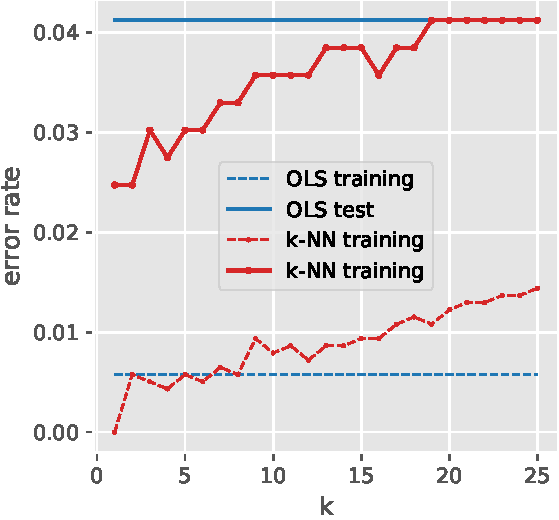
\includegraphics[width=\half]{E2p8_A.pdf}
\end{minipage}\halfspace
\begin{minipage}{\half}
\centering
\begin{tabular}{|c|c|c|}
\hline
\textbf{Model} & \textbf{Training error} & \textbf{Test error}\\
\hline
OLS & 0.58 \% & 4.12 \% \\
\hline
1-NN & 0 & 2.47 \% \\
\hline
3-NN & 0.50 \% & 3.02 \% \\
\hline
5-NN & 0.58 \% & 3.02 \% \\
\hline
7-NN & 0.65 \% & 3.30 \% \\
\hline
15-NN & 0.94 \% & 3.85 \% \\
\hline
\end{tabular}
\end{minipage}



\subsection*{Ex. 2.9}
Let's denote $R(Z_{tr}, Z_{te})$ the average of squared residuals for $Z_{te}$ using the OLS coefficients from $Z_{tr}$. Using the notation from the exercise:
\begin{eqnarray*}
R_{tr}(\hat{\beta}) \equiv R(Z_{tr}, Z_{tr}), \qquad R_{te}(\hat{\beta}) \equiv R(Z_{tr}, Z_{te})
\end{eqnarray*}
It is easy to verify that the expected value $ \mathbb{E}_{Z_{te}} \left[ R(Z_{tr}, Z_{te}) \right]$ does not depend on $M \equiv |Z_{te}|$ (assuming the test examples are i.i.d.). This allows us to take $M = N$. Now, by definition of OLS estimates we have:
\begin{eqnarray*}
R(Z_{te}, Z_{te}) \leq R(Z_{tr}, Z_{te})
\end{eqnarray*}
Now that $M = N$, the lhs has the same distribution as $R(Z_{tr}, Z_{tr})$, so when taking the expectation value:
\begin{eqnarray*}
\mathbb{E}_{Z_{te}, Z_{tr}} \left[ R(Z_{tr}, Z_{tr}) \right] = \mathbb{E}_{Z_{te}, Z_{tr}} \left[ R(Z_{te}, Z_{te}) \right] \leq \mathbb{E}_{Z_{te}, Z_{tr}} \left[ R(Z_{tr}, Z_{te})  \right]
\end{eqnarray*}
which proves the assertion.
% !TeX root = Tibt.tex

\section*{Chapter 3: Linear methods for regression}

\subsection*{Ex. 3.1}
We can use the results from Section 3.2.3 to prove the statement for the last predictor $j = p$. This generalizes for all other predictors, since neither the $z$-score nor the $F$-statistic depend on the order of predictors.

Letting $ \mathbf{z}_j$ be the columns of $Z$ as in Eq. (3.30) in the text and assuming additive gaussian errors, 
we have the following:
\begin{eqnarray*}
\textrm{Var}(\hat{\beta}_p) & = & \frac{\sigma^2}{|| \mathbf{z}_p||^2} \qquad \textrm{(Eq. (3.29) in the text)}\\
\mathbf{z_j} \cdot \mathbf{z_k} & = & 0 \quad \textrm{for } j \neq k
\end{eqnarray*}
The $z$-score for predictor $j$ had been defined (see Eq. (3.12) in the text) as the ratio between the OLS value $\hat{\beta}_j$
and the square root of the estimate of $\textrm{Var}(\hat{\beta}_p)$ obtained by replacing $\sigma$ with $\hat{\sigma}$, hence:
\begin{eqnarray*}
z_p^2 & \equiv & \frac{\hat{\beta}_p^2}{\hat{\sigma}^2 / || \mathbf{z}_p||^2}
\end{eqnarray*}
Adopting the notation used to defined the $F$-score in Eq. (3.13) in the text:
\begin{eqnarray*}
\hat{\sigma}^2 = \frac{\textrm{RSS}_1}{N - p - 1}
\end{eqnarray*}
where $\textrm{RSS}_1$ is the sum of squared residuals when the $p$-th predictor is included. We have then:
\begin{eqnarray*}
z_p^2 = \frac{\hat{\beta}_p ^2\,|| \mathbf{z}_p||^2}{\textrm{RSS}_1 / (N - p - 1)}
\end{eqnarray*}
Since $\mathbf{z}_p$ is orthogonal to all other predictors, it is easy to check that:
\begin{eqnarray*}
\textrm{RSS}_1 = \textrm{RSS}_0 - \hat{\beta}_p^2 \, || \mathbf{z}_p ||^2
\end{eqnarray*}
Hence, according to Eq. (3.13) in the text:
\begin{eqnarray*}
F_{p} \equiv \frac{\textrm{RSS}_0 - \textrm{RSS}_1}{\textrm{RSS}_1 / (N - p - 1)} = \frac{\hat{\beta}_p^2 \, || \mathbf{z}_p ||^2}{\textrm{RSS}_1 / (N - p - 1)} = z_p^2
\end{eqnarray*}

\subsection*{Ex. 3.2 \seecode}
The premise of the two confidence band estimates is that the posterior
distribution of the true value $\beta$ given the data is that of a gaussian vector, 
with center $\hat{\beta}$ and covariance $ \hat{\sigma}^2 \left( \mathbf{X} ^T \mathbf{X}  \right) ^{-1}$. In the case described by the exercise $\mathbf{X}$
is the matrix whose columns contains increasing powers of the samples of $X$.
The two confidence bands are then obtained as follows:
\begin{enumerate}
\item Since $\beta^T x_0$ is also gaussian with mean $\hat{y}_0 \equiv \hat{\beta}^T x_0$ and variance $\hat{\sigma}^2\, x_0^T ( \mathbf{X} ^T \mathbf{X})^{-1} x_0$, we can define a confidence band for its value via:
\begin{eqnarray*}
\mathcal{C}_1 =  \left\{ y \; : \; (y - \hat{y}_0)^2 \leq \hat{\sigma}^2 \, x_0^T ( \mathbf{X} ^T \mathbf{X})^{-1} x_0 \, {\chi_{1}^2} ^{\,(1- \alpha)} \right\}
\end{eqnarray*}
where ${\chi_{1}^2} ^{\,(1- \alpha)}$ is the $1 - \alpha$ percentile of a chi-squared distribution with one degree of freedom, i.e. the distribution of the squared of a normal random variable:
\begin{eqnarray*}
P(\beta^T x_0 \in \mathcal{C}_1 \, | \, Y) = 1 - \alpha
\end{eqnarray*}
\item One has (cf. Eq. (3.15) in the text):
\begin{eqnarray*}
( \hat{\beta} - \beta) ^T \, \mathbf{X}^T \mathbf{X} \, ( \hat{\beta} - \beta) \sim \hat{\sigma}^2 \chi_{p+1}^2
\end{eqnarray*}
We can thus define a confidence interval for the whole vector $\beta$ as:
\begin{eqnarray*}
&& \mathcal{C}_{2, \beta}  = \left\{ \beta \; : \;\frac{1}{\hat{\sigma}^2} ( \hat{\beta} - \beta) ^T \, \mathbf{X}^T \mathbf{X} \, ( \hat{\beta} - \beta) \leq  {\chi_{p + 1}^2} ^{\,(1- \alpha)} \right\} \\
&& P(\beta \in \mathcal{C}_{2, \beta} \, | \, Y)  =  1 - \alpha
\end{eqnarray*}
This in turns generate a confidence interval for $\beta^T x_0$ as:
\begin{eqnarray*}
\mathcal{C}_2 = \left\{ y = \beta^T x_0: \; \beta \in \mathcal{C}_{2, \beta} \right\}
\end{eqnarray*}
\end{enumerate}
The two confidence bands are very much related, as we now show. First, one can easily show that both $\mathcal{C}_1$ and $\mathcal{C}_2$
do not change if we start with a different set of predictors, related to the original ones via a non-singular linear
transformation. Hence, we can assume that the predictors are orthogonal and normalised, $ \mathbf{X}^T \mathbf{X} = \mathbb{I}_p$. We then have:
\begin{eqnarray}\label{3p2_e1}
\mathcal{C}_1 = \left\{ y\; : \; (y - \hat{y}_0)^2 \leq \hat{\sigma}^2\, ||x_0||^2\, {\chi_{1}^2} ^{\,(1- \alpha)} \right\}
\end{eqnarray}
and:
\begin{eqnarray*}
\mathcal{C}_{2, \beta} = \left\{ \beta \; : \; || \hat{\beta} - \beta ||^2 \leq \hat{\sigma}^2 {\chi_{p + 1}^2} ^{\,(1- \alpha)} \right\}
\end{eqnarray*}
or equivalently:
\begin{eqnarray*}
	\mathcal{C}_{2, \delta \beta} & \equiv & \left\{ \delta \beta \; : \; || \delta \beta || ^2 \leq  \hat{\sigma}^2 \, {\chi_{p + 1}^2} ^{\,(1- \alpha)} \right\} \\
\mathcal{C}_2 & = & \left\{ y = \hat{y}_0 + \delta \beta^T x_0: \; \delta \beta \in \mathcal{C}_{2, \delta \beta} \right\} 
\end{eqnarray*}
One can easily prove that $\mathcal{C}_2$ is, like $\mathcal{C}_1$, an interval centered around $\hat{y_0}$. Finding its upper limit corresponds to solving:
\begin{eqnarray*}
\textrm{max} \, \delta \beta^T x_0 \quad \textrm{on} \quad || \delta \beta || ^2 \leq  \hat{\sigma}^2 \, {\chi_{p + 1}^2}^{\,(1- \alpha)}
\end{eqnarray*}
The solution is:
\begin{eqnarray*}
\textrm{max} \, \delta \beta^T x_0 = \left(  \hat{\sigma}^2 ||x_0||^2 \, {\chi_{p + 1}^2}^{\,(1- \alpha)}  \right) ^{1/2}
\end{eqnarray*}
Hence:
\begin{eqnarray} \label{3p2_e2}
\mathcal{C}_2 = \left\{ y \; : \; (y - \hat{y}_0)^2 \leq \hat{\sigma}^2 ||x_0||^2 \, {\chi_{p + 1}^2}^{\,(1- \alpha)} \right\}
\end{eqnarray}
Comparing (\ref{3p2_e2}) with (\ref{3p2_e1}) we see that:
\begin{eqnarray}
\frac{\textrm{diam}^2(\mathcal{C}_2)}{\textrm{diam}^2(\mathcal{C}_1)} = \frac{{\chi_{p + 1}^2}^{\,(1- \alpha)}}{{\chi_{1}^2}^{\,(1- \alpha)}} \geq 1
\end{eqnarray}
The equality holds only for $p = 0$, i.e. when we only fit a constant, or more generally with only a single predictor. So, the point-wise confidence bands are narrower.

We can also provide a simple graphical interpretation for this result. First, notice that the size of both confidence
intervals scales linearly with $||x_0||$, hence to get an idea of interval sizes we can set $||x_0|| = 1$.
The quantity $\beta^T x_0$ can now be interpreted as the euclidean projection of the random $\beta$ vector
onto the unit vector $x_0$. Using orthonormal predictors, the confidence band size is independent on the direction
of $x_0$ (see (\ref{3p2_e2}) and (\ref{3p2_e1})) and we can set $x_0 = e_1$, hence $\beta^T x_0 = \beta_1$. With this
choice, we see that the first confidence band estimate corresponds to a band $\{|\beta_1 - \hat{\beta}_1| \leq c \}$ with probability $1 - \alpha$. On the other hand, the second choice consists in finding a ball in the $\beta$ space with the same probability, then to project this set onto the $e_1$ axis. It is then obvious that the ball diameter needs
to be wider than  previous band-sized set in order for their probabilities to be the same (see Figures \ref{3p2_f1} and \ref{3p2_f2}).

\hspace{0.5cm}\\
\begin{figure}
\begin{minipage}{\half}
	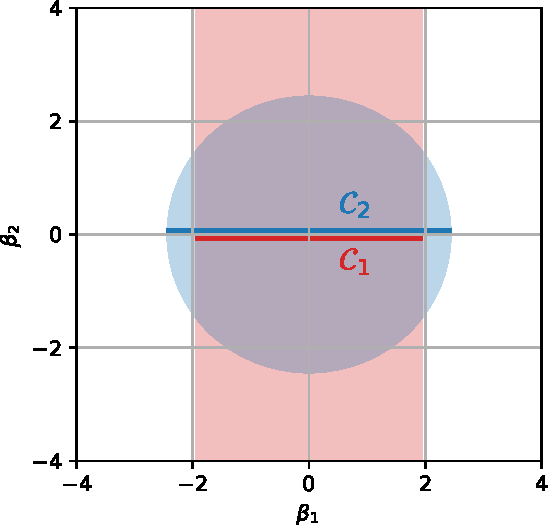
\includegraphics[width=\half]{E3p2_A.pdf} \caption{Confidence bands: single projection versus full vector.
		The two-dimensional vector $\beta$ is taken to be centered and to have unit covariance. Both highlighted areas
		have $95\%$ probability, but the band-shaped one has smaller projection on the $\beta_1$ axis. \label{3p2_f1}}

\end{minipage}\halfspace
\begin{minipage}{\half}
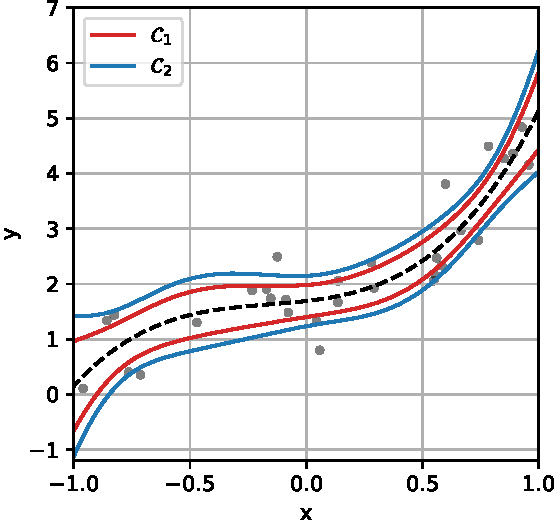
\includegraphics[width=\half]{E3p2_B.pdf} \caption{Confidence bands for a cubic univariate model. Values of $x$ have
	been drawn from a uniform distribution in $[-1, 1]$, and $y$ has been generated as $\beta^T x^{(3)} + \epsilon$,
	where $\beta$ is a centered, unit-covariance gaussian vector, $x^{(3)} \equiv (1, x, x^2, x^3)$ and $\epsilon$
	is a centered gaussian with variance equal to $0.25$. \label{3p2_f2}}
\end{minipage}
	\end{figure}

\subsection*{Ex. 3.3}
Any linear, unbiased estimate $c^T Y$ of $a^T \beta$ can be written as the OLS estimator
plus an additional linear estimate with zero expectation:
\begin{eqnarray*}
&& c^T Y \equiv  a^T \hat{\beta} + b^T Y = \left( a^T \left( \mathbf{X}^T \mathbf{X} \right)^{-1} \mathbf{X}^T + b^T \right) Y \\
&& \mathbb{E} \left[ b^T Y \right] = b^T \mathbf{X} \beta = 0
\end{eqnarray*}
Since the second equation must hold for any $\beta$, we conclude $ b^T \mathbf{X} = 0$. This implies that
the two terms in:
\begin{eqnarray*}
c = \mathbf{X} \left( \mathbf{X} ^T \mathbf{X}  \right)^{-1} a + b
\end{eqnarray*}
are orthogonal vectors. Hence, the variance:
\begin{eqnarray*}
\textrm{Var} \left( c^T Y \right) & = & \sigma^2 ||c||^2
\end{eqnarray*}
is minimized for $b=0$, i.e. when $c^T Y = a^T \hat{\beta}$.

Similarly, any linear unbiased estimate $C^T Y$ of the $\beta$ vector can be written as:
\begin{eqnarray} \nonumber
C^T Y & = & \left( \left( \mathbf{X}^T \mathbf{X} \right)^{-1} \mathbf{X} ^T + B^T \right) Y \equiv \left(  \hat{B} + B \right)^T Y\\ \label{3p3_e1}
B^T \mathbf{X} & = & 0 \quad \Longrightarrow \quad B^T \hat{B} = 0
\end{eqnarray}
Its variance-covariance matrix is:
\begin{eqnarray*}
\textrm{Cov}(C^T Y)  =  C^T C = \hat{B}^T \hat{B} + B^T B
\end{eqnarray*}
where the last equality follows from (\ref{3p3_e1}). Since $B^T B$ is positive semi-definite,
this proves that:
\begin{eqnarray*}
\textrm{Cov}(\hat{\beta}) = \hat{B}^T \hat{B} \lesssim \textrm{Cov}(C^T Y)
\end{eqnarray*}

\subsection*{{\color{red} Ex. 3.4}}
Using the QR decomposition $\mathbf{X} = \mathbf{Q}_{Np} R_{pp}$, $\mathbf{Q}^T \mathbf{Q} = \mathbb{I}$, we see that:
\begin{eqnarray*}
\hat{\beta} & = & \left( \mathbf{X} ^T \mathbf{X} \right)^{-1} \mathbf{X}^T \mathbf{y} = R^{-1} \mathbf{Q}^T \mathbf{y} \equiv R^{-1} \hat{\beta}^q\\
\hat{\beta}^q & \equiv & \mathbf{Q}^T \mathbf{y}
\end{eqnarray*}
This identity can be given a procedural interpretation via the Gram-Schmidt procedure.

\begin{enumerate}
	\item Start with $\hat{\beta} = 0$.
	\item For $j = 1, \ldots, p$:
	\begin{itemize}
		\item Compute the $j$-th column $\mathbf{q}_j$ of Q, and the $j$-th column of R as per
			the Gram-Schmit procedure. This corresponds to:
			\begin{eqnarray*}
			\mathbf{x}_j & = & R_{1j} \mathbf{q}_1 + \ldots + R_{jj} \mathbf{q}_j
			\end{eqnarray*}
			where $\mathbf{q}_j$ satisfies $\langle \mathbf{q}_i, \mathbf{q}_j \rangle = \delta_{ij}$.
		\item Compute the regression coefficient $\hat{\beta}_j^q$ of $\mathbf{y}$ against $\mathbf{q}_j$
			as $\langle \mathbf{q}_j, \mathbf{y} \rangle$. Notice that, the $\mathbf{q}_j$'s being orthogonal,
			$\hat{\beta}_j^q$ is the coefficient of $\mathbf{q}_j$ in the regression of $\mathbf{y}$ against
			all of the $\mathbf{q}_j$'s:
			\begin{eqnarray*}
				\mathbf{y} & \sim & \hat{\beta}^q_1\, \mathbf{q}_1 + \ldots + \hat{\beta}^q_p\, \mathbf{q}_p
			\end{eqnarray*}
		\item Compute the $j$-th column of $R^{-1}$ via backward substitution. Notice that this only 
		requires the first $j$ columns of $R$, which are available at this stage. We have then:
		\begin{eqnarray}
		\label{3p4_e1}
		\mathbf{q}_j & = & (R^{-1})_{1j}\,\mathbf{x}_1 + \ldots + (R^{-1})_{jj}\, \mathbf{x}_j
		\end{eqnarray}
		\item Update the coefficients of the original predictors according to the new term in the regression:
		\begin{eqnarray*}
		\hat{\beta}^q_j\, \mathbf{q}_j & = & \hat{\beta}^q_j \left( (R^{-1})_{1j}\,\mathbf{x}_1 + \ldots + (R^{-1})_{jj}\, \mathbf{x}_j \right)\\
		\hat{\beta}_i &\rightarrow& \hat{\beta}_i + (R^{-1})_{ij}\,\hat{\beta}^q_j \quad i = 1,\ldots,j
		\end{eqnarray*}
	\end{itemize}
\end{enumerate}

\subsection*{Ex. 3.5}
One has:
\begin{eqnarray*}
\beta_0 + \sum_j x_{ij} \beta_j & = & \beta_0^c + \sum_j (x_{ij} - \bar{x}_j) \beta_j \\
\beta_0^c & \equiv & \beta_0 + \sum_j \bar{x}_j \beta_j
\end{eqnarray*}
Since $\beta_0$ is a dummy variable in the OLS minimization, we can use $\beta_0^c$ instead,
which proves the equivalence and provides the relationship between $\beta$ and $\beta^c$:
\begin{eqnarray*}
\beta_0^c & = & \beta_0 + \sum_j \bar{x}_j \beta_j \\
\beta_j^c & = & \beta_j, \quad j = 1, \ldots, p
\end{eqnarray*}

As a side note, this shows that as long as we include the constant in a Ridge regression,
we should not worry about the remaining predictors being centered: their average
can be absorbed in the coefficient of the constant which is not penalized.

\subsection*{Ex. 3.6}
From Bayes theorem:
\begin{eqnarray*}
P_{posterior}(\beta | \mathbf{y}) \propto P(\mathbf{y} | \beta) \, P_{prior}(\beta)
\end{eqnarray*}
The proportionality factor only depends on $\mathbf{y}$ and is fixed by the normalization of
the posterior distribution. Assuming\footnote{The text exercise uses $\tau$ instead of $\tau^2$. This 
seems inconsistent with the next exercise and with the convention for variances, so we use $\tau^2$ instead.}:
\begin{eqnarray*}
l_{prior}(\beta) & \equiv & \log{P_{prior}(\beta)} = c_1 - \frac{1}{2 \tau ^2} \beta^T \beta\\
\log{P(\mathbf{y} | \beta)} & = & c_2 - \frac{1}{2 \sigma^2} \left( \mathbf{y} - \mathbf{X} \beta \right)^T \left( \mathbf{y} - \mathbf{X} \beta \right) 
\end{eqnarray*}
we get:
\begin{eqnarray} \label{3p6_e1}
l_{posterior}(\beta | \mathbf{y}) & = & c_3 - \frac{1}{2 \tau^2} \beta^T \beta - \frac{1}{2 \sigma^2} \left( \mathbf{y} - \mathbf{X} \beta \right)^T \left( \mathbf{y} - \mathbf{X} \beta \right) \\ \nonumber
& = & c(\mathbf{y}) - \frac{1}{2} \left( \beta - \hat{\beta} \right) ^T \left( \frac{\mathbf{X} ^T \mathbf{X} }{ \sigma ^2} + \frac{1}{\tau^2} \right) \left( \beta - \hat{\beta} \right) \\ \nonumber
\hat{\beta} & = & \left( \mathbf{X} ^T \mathbf{X} + \frac{\sigma^2}{ \tau^2} \right)^{-1} \mathbf{X}^T \mathbf{y}
\end{eqnarray}
This shows that the posterior distribution of $\beta$ is gaussian, with center given by the Ridge estimate
with parameter $\lambda = \sigma^2 / \tau^2$.

\subsection*{Ex. 3.7}
This is almost equivalent to (\ref{3p6_e1}), which was derived in the previous exercise.
The only difference is the presence of the constant $\beta_0$. In the absence of a prior for $\beta_0$,
the expression in the exercise:
\begin{eqnarray*}
\sum_{i=1}^N \left( y_i -\beta_0 \sum_j x_{ij} \beta_j \right)^2 + \lambda \sum_j \beta_j^2
\end{eqnarray*}
is not a valid log-likelihood for $\beta \equiv (\beta_j)_{j=1,\ldots,p}$, since $\beta_0$ remains
unspecified. Two possibilities come to mind: first, that $\beta_0$ is deterministic ($\tau_0 = 0$) 
and known in advance, in which case (\ref{3p6_e1}) yields the results in the exercise
when we replace $\mathbf{y}$ by $\mathbf{y} - \beta_0$. 

The second, more likely possibility is that we have no prior on $\beta_0$. This can be modelled as
a gaussian prior with $\tau_0 \rightarrow \infty$, in which case we can repeat the steps of the 
previous exercise to get:
\begin{eqnarray*}
l_{posterior}(\beta, \beta_0 | \mathbf{y}) = c - \frac{1}{2 \tau_0^2} \beta_0^2 - \frac{1}{2 \tau^2} \beta^T \beta - \frac{1}{2 \sigma^2} \left( \mathbf{y} - \beta_0 - \mathbf{X} \beta \right)^T \left( \mathbf{y}- \beta_0 - \mathbf{X} \beta \right)
\end{eqnarray*}
Since we are interested in the posterior distribution for $\beta$, we should integrate over $\beta_0$ the exponential of $l_{posterior}(\beta, \beta_0 | \mathbf{y})$. As $\tau_0 \rightarrow \infty$, one can
show that upon integration:
\begin{eqnarray*}
	l_{posterior}(\beta | \mathbf{y}) & = & c(\mathbf{y}) - \frac{1}{2 \tau^2} \beta^T \beta - \frac{1}{2 \sigma^2} \left( \mathbf{y} - \mathbf{X} \beta \right)^T \left( \mathbb{I} - \frac{e e^T}{N} \right)\left( \mathbf{y}  - \mathbf{X} \beta \right) \\
	& = & c(\mathbf{y}) - \frac{1}{2 \tau^2} \beta^T \beta - \frac{1}{2 \sigma^2} \left( \mathbf{y}_c - \mathbf{X}_c \beta \right)^T \left( \mathbf{y}_c  - \mathbf{X}_c \beta \right)
\end{eqnarray*}
where $\mathbf{y}_c$ and $\mathbf{X}_c$ are the centered versions of $\mathbf{y}$ and $\mathbf{X}$.

\subsection*{Ex. 3.8}}

We begin by proving that $\mathbf{Q}_2$ is the 'Q' matrix in
the QR decomposition of $\tilde{\mathbf{X}}$.
Denote $(\mathbf{q}_0 = \mathbf{e}, \mathbf{q}_1, \ldots, \mathbf{q}_p)$ the 
columns of $\mathbf{Q}$, the matrix appearing in the QR decomposition $\mathbf{X}$. The matrix $\mathbf{Q}_2$ has columns $(\mathbf{q}_1, \ldots, 
\mathbf{q}_{p})$. The centered matrix $\tilde{\mathbf{X}}$ can be written as:

\begin{equation}
\tilde{\mathbf{X}} = \left(\mathbf{X} - \frac{1}{N} \mathbf{e}\, \mathbf{e}^T\mathbf{X}\right) E_{p+1, p}
\end{equation}
where $E_{p + 1, p}$ is the $(p + 1) \times p$ matrix containing
an identity block starting at position $(1, 0)$, so as to remove
the first column of the matrix on its left.
Replacing the QR decomposition of $\mathbf{X}$ we get:
\begin{equation}
\tilde{\mathbf{X}} = \left(\mathbb{I}_{p+1, p + 1} - \frac{1}{N} \mathbf{e}\,\mathbf{e}^T\right) \mathbf{Q}\,R\, E_{p+1, p}
\end{equation}
Since $\mathbf{q}_0 = \mathbf{e}$ and the remaining columns of $\mathbf{q}$
are orthogonal to $\mathbf{e}$ as per the Gram-Schmidt procedure, the first
term on the r.h.s. has the effect of multiplying by zero the first column of
$\mathbf{Q}$ while leaving the remaining columns $\mathbf{Q}_2$ untouched:
\begin{equation}
\tilde{\mathbf{X}} = \mathbf{Q}_2\, E_{p, p+1} \,R\, E_{p+1, p}
\end{equation}
where $E_{p, p+1}$ is the $p \times (p + 1)$ matrix containing an identity
block starting at index $(0, 1)$. The matrix $E_{p, p+1} \,R\, E_{p+1, p}$
is nothing but the $1$ to $p + 1$ submatrix of $R$, which is still upper diagonal.
This proves that $\mathbf{Q}_2$ is the 'Q' matrix in the QR decomposition of
$\tilde{\mathbf{X}}$.

Let now $\tilde{\mathbf{X}} = UDV^T$. Since $DV^T$ is a non-singular $p \times p$
matrix, the columns of $U$ must span the same subspace as the columns of both
$\tilde{\mathbf{X}}$ and $\mathbf{Q}_2$. From now on we can drop both the tildes
and the subscript, since both the QR and SVD decompositions are performed
on the centered matrix.

For the second part of the question we note that, if the columns of 
$\mathbf{X}$ are mutually orthogonal, the QR decomposition is also
an SVD decomposition, because the $R$ matrix can be taken to be diagonal:

\begin{eqnarray*}
    \mathbf{X} & = & \mathbf{Q} D \\
    D_{kk} & = & ||\mathbf{x}_k|| \\
    \mathbf{Q}^T \mathbf{Q} & = & \mathbb{I}_p
\end{eqnarray*}
Since the SVD is unique\footnote{Here we suppose that the eigenvalues of
the sample covariance matrix are all distinct.} up to shuffling and sign flip
of the columns of $\mathbf{U}$, the matrix $\mathbf{Q}$ can be obtained from
any of the versions of $\mathbf{U}$ using such operations. One can in fact show that 
this is the only case in which the columns of $\mathbf{Q}$
coincide those of $\mathbf{U}$. Suppose that:
\begin{equation*}
\mathbf{Q} = \mathbf{U}
\end{equation*}
By comparing the two decompositions one can easily show that:
\begin{equation*}
V = D^{-1} R
\end{equation*}
This equality requires $V$ to be upper-diagonal besides being orthogonal. This
implies\footnote{Any upper-diagonal orthogonal matrix $V$ is necessarily diagonal. To
show this, one can prove that $V^{-1}$ is also upper-diagonal and, being
equal to the transpose $V^T$, $V$ must be diagonal.} that $V$ is a diagonal, idempotent matrix, and:
\begin{equation*}
\mathbf{X}^T \mathbf{X} = V^T D ^2 V
\end{equation*}
is also diagonal, proving that the columns of $\mathbf{X}$ are mutually orthogonal.

\subsection*{Ex. 3.9}
If we add a new predictor $\mathbf{z}$ to the fit, the residual-sum-of squares changes by:
\begin{eqnarray*}
RSS \; \longrightarrow \; RSS - \left( \frac{ \langle \mathbf{y}, \mathbf{z}^{(r)} \rangle}{||\mathbf{z}^{(r)} ||} \right) ^2
\end{eqnarray*}
where $ \mathbf{z}^{(r)}$ is the OLS residual of $ \mathbf{z}$ against the predictors already included in the fit, $\mathbf{X}_1$ in this case. Hence, it suffices to find the matrix $\mathbf{X}_{2}^{(r)}$ of residuals,
which is easy to compute using the QR decomposition $\mathbf{X}_1 =  \mathbf{Q}R$:
\begin{eqnarray} \label{3p9_e0}
\mathbf{X}_{2}^{(r)} & = & \mathbf{X}_2 - \mathbf{X}_1 \left( \mathbf{X}_1^T \mathbf{X}_1 \right)^{-1} \mathbf{X}_1^T \mathbf{X}_2 \\
& = & \left( \mathbb{I} - \mathbf{Q} \mathbf{Q}^T \right) \mathbf{X}_2
\end{eqnarray}
Then, we choose the predictor $\mathbf{x}_{2, \bar{j}}$ such that:
\begin{eqnarray} \label{3p9_e1}
\bar{j} = \textrm{argmax}\, \frac{| \langle \mathbf{y}, \mathbf{x}_{2, j}^{(r)} \rangle |}{||\mathbf{x}_{2, j}^{(r)}||} = \textrm{argmax}\, \frac{| \langle \mathbf{r}, \mathbf{x}_{2, j}^{(r)} \rangle |}{||\mathbf{x}_{2, j}^{(r)}||} = \textrm{argmax}\, \frac{| \langle \mathbf{r}, \mathbf{x}_{2, j} \rangle |}{||\mathbf{x}_{2, j}^{(r)}||}
\end{eqnarray}
The last two equalities follows from the fact that, by construction, $\mathbf{x}_{2, j}^{(r)}$ and $\mathbf{r}$ are orthogonal to the subspace generated by the columns of $\mathbf{X}_1$, hence to $\hat{\mathbf{y}} = \mathbf{y} - \mathbf{r}$ and $\mathbf{x}_{2, j} - \mathbf{x}_{2, j}^{(r)}$. The
process can be continued by adding the column $\mathbf{x}_{2, \bar{j}}^{(r)} / ||\mathbf{x}_{2, \bar{j}}^{(r)}||$ to $Q$, and updating R according to (\ref{3p9_e0}).

Note how one has generally $||\mathbf{x}_{2, j}^{(r)}|| \leq ||\mathbf{x}_{2, j}||$, the equality holding 
only when $\mathbf{x}_{2, j}$ is orthogonal to $\mathbf{X}_1$. Hence, the criterion (\ref{3p9_e1}) is not equivalent to:
\begin{eqnarray} \label{3p9_e2}
\bar{j} = \textrm{argmax}\, \frac{| \langle \mathbf{r}, \mathbf{x}_{2, j} \rangle |}{||\mathbf{x}_{2, j}||}
\end{eqnarray}
Indeed, in forward stepwise regression we allow ourselves to change the coefficients of the predictors in the
current active set $ \mathbf{X}_1$, so as to only pick the "new" part in $\mathbf{x}_{2, j}$. Conversely, criterion (\ref{3p9_e2}), which corresponds to forward stagewise regression, tends to penalize predictors
which are strongly correlated with the predictors in the active set.

\subsection*{Ex. 3.10}
In Exercise 3.10, we established that the $F$-score for dropping a single predictor equals the square
of the corresponding $z$-score. Since the $F$ score is proportional to the increase in residual-sum-of 
squares when the predictor is dropped, we see that the predictor with smallest absolute $z$-score is be the one to be dropped.

\subsection*{Ex. 3.11}
Note that:
\begin{eqnarray*}
\textrm{RSS}(B) = \textrm{Tr} \left(\Sigma^{-1} \left( \mathbf{Y} - \mathbf{X} B \right)^T \left( \mathbf{Y} - \mathbf{X} B \right)\right)
\end{eqnarray*}
When the matrix $\Sigma$ is diagonal, this is a sum of $K$ independent RSS's, and the solution for
$B$ is indeed:
\begin{eqnarray} \label{3p11_e0}
B = \left( \mathbf{X} ^T \mathbf{X} \right)^{-1} \mathbf{X} \mathbf{Y}
\end{eqnarray}
More generally, since $\mathbf{\Sigma}$ is symmetric and positive definite, it admits a square root $S$, which allows us to fall back on the diagonal case:
\begin{eqnarray*}
\textrm{RSS}(B) & = & \textrm{Tr} \left(\left( \mathbf{\hat{Y}} - \mathbf{X} \hat{B} \right)^T \left( \mathbf{\hat{Y}} - \mathbf{X} \hat{B} \right)\right)\\
\mathbf{\hat{Y}} & \equiv &\mathbf{Y}\,S\\
\hat{B} & \equiv & B\, S
\end{eqnarray*}
Hence the OLS solution is given by:
\begin{eqnarray*}
B = \hat{B}\, S^{-1} = \left( \mathbf{X} ^T \mathbf{X} \right)^{-1} \mathbf{X} \hat{\mathbf{Y}} \, S^{-1} = \left( \mathbf{X} ^T \mathbf{X} \right)^{-1} \mathbf{X} \mathbf{Y}
\end{eqnarray*}

When the matrix $\Sigma$ varies from instance to instance, the value of $B$ which minimizes $\textrm{RSS}$
is no longer given by a simple formula like (\ref{3p11_e0}). However, $\textrm{RSS}$ is still a quadratic
form in $B$, seen as a vector in $\mathbb{R}^{p \times K}$. So, the equation which determines $B$ 
can be shown to be an affine equation:
\begin{eqnarray*}
&& \sum_{(k, b)} L_{(j, a), (k, b)} \, B_{(k, b)} - C_{j, a} = 0\\
&& L_{(j, a), (k, b)} = \sum_i \Sigma^{-1}_{i, ab} \, X_{ij}\, X_{ik}\\
&& C_{j, a} = \sum_{i, b} \Sigma^{-1}_{i, ab} \, X_{ij} Y_{ib}
\end{eqnarray*}
This can be solved using standard linear system methods.

\subsection*{Ex. 3.12}
Denote by $\mathbf{X}_a$ and $\mathbf{y}_a$ the matrices $\mathbf{X}$ and $\mathbf{y}$ after the indicated
rows have been added. One has:
\begin{eqnarray*}
\mathbf{X}_a^T \mathbf{X}_a & = & \left( \begin{array}{cc}  \mathbf{X}^T  & \sqrt{\lambda}\, \mathbb{I}  \end{array}\right) \left( \begin{array}{c} \mathbf{X} \\ \sqrt{\lambda}\, \mathbb{I} \end{array} \right) = \mathbf{X}^T \mathbf{X} + \lambda \mathbf{I}\, \mathbb{I} \\
\mathbf{X}_a^T \mathbf{Y}_a & = & \left( \begin{array}{cc}  \mathbf{X}^T  & \sqrt{\lambda}\, \mathbb{I}  \end{array}\right) \left( \begin{array}{c} \mathbf{y} \\ 0 \end{array} \right) = \mathbf{X}^T \, \mathbf{y}
\end{eqnarray*}
therefore $\hat{\beta}_a = \left( \mathbf{X}_a^T \mathbf{X}_a \right)^{-1} \mathbf{X}_a^T \mathbf{y} =  \left( \mathbf{X}^T \mathbf{X} + \lambda \mathbf{I} \right)^{-1} \mathbf{X}^T \mathbf{y} = \hat{\beta}_{r}(\lambda)$.

\subsection*{Ex. 3.13}
After centering predictors, the PCR fitted function is:
\begin{eqnarray*}
\hat{f}(x) = \bar{y} +\sum_{m=1}^M \hat{\theta}_m \, z_m = \bar{y} + \sum_{m=1}^M \hat{\theta}_m \, (x \cdot v_m) = \bar{y} + \left( \sum_{m=1}^M \hat{\theta}_m \, v_m\right) \cdot x = \bar{y} + \hat{\beta}^{pcr} \cdot x
\end{eqnarray*} 
which proves the first point.

The proof of the second point follows from the fact that the span of the $\mathbf{x}$'s is equal to
the span of all the $\mathbf{z}$'s. Remembering that $\mathbf{X} = \mathbf{Z}V^T$ where $\mathbf{z}_m$ are the columns of $\mathbf{Z}$ and $V$ is orthogonal:
\begin{eqnarray*}
\hat{\beta}^{ls}  =  \left( \mathbf{X}^T \mathbf{X} \right)^{-1} \mathbf{X}^T \mathbf{y} =
 V \left( \mathbf{Z}^T \mathbf{Z} \right)^{-1} \mathbf{Z}^T \mathbf{y}
\end{eqnarray*}
Since the columns of $\mathbf{Z}$ are orthogonal, this reads:
\begin{eqnarray*}
\hat{\beta}^{ls} & = & \sum_{m=1}^{p} \frac{\langle \mathbf{z}_m, \mathbf{y} \rangle}{\langle \mathbf{z}_m, \mathbf{z_m} \rangle} \, v_m = \hat{\beta}^{pcr}(p)
\end{eqnarray*}

\subsection*{Ex. 3.14}
When predictors are orthogonal and normalised ($\langle \mathbf{x}_j, \mathbf{x}_k \rangle = N \, \delta_{jk}$), the vector $\hat{\theta}_1 \, \mathbf{z}_1$ found at the first step of the PLS procedure is the orthogonal projection of $\mathbf{y}$ on the span of the $\mathbf{x}$'s:
\begin{eqnarray*}
\mathbf{z}_1 & = & \sum_{j=1}^p \langle \mathbf{x}_j, \mathbf{y} \rangle\, \mathbf{x}_j\\
\hat{\theta}_1 & = & \frac{\langle \mathbf{z}_1, \mathbf{y} \rangle}{\langle \mathbf{z}_1, \mathbf{z}_1 \rangle} = \frac{\sum_{j=1}^p \langle \mathbf{x}_j, \mathbf{y} \rangle ^2}{N \sum_{j=1}^p \langle  \mathbf{x}_j, \mathbf{y} \rangle ^2} = 1/N\\
\hat{\theta}_1 \mathbf{z}_1 & = & \sum_{j=1}^p \frac{\langle \mathbf{x}_j, \mathbf{y} \rangle}{N} \, \mathbf{x}_j = \sum_{j=1}^p \frac{\langle \mathbf{x}_j, \mathbf{y} \rangle}{\langle \mathbf{x}_j, \mathbf{x}_j \rangle} \, \mathbf{x}_j = \hat{\mathbf{y}}^{ls}
\end{eqnarray*}
In other words, at step $m = 1$ we find the OLS fit of $\mathbf{y}$ against the $\mathbf{x}$'s. In preparation
for the next step, the $\mathbf{x}_j$ are residualised against $\mathbf{z}_1$: we obtain a set of vectors
$\mathbf{x}_j^{(1)}$ which still lie in the span of the $\mathbf{x}$'s, but are orthogonal to the projection
of $\mathbf{y}$ onto the same subspace. Therefore, at the next step, we'll have:
\begin{eqnarray*}
\hat{\varphi}_{2j} = \langle \mathbf{x}_{j}^{(1)}, \mathbf{y} \rangle =  \langle \mathbf{x}_{j}^{(1)}, \hat{\mathbf{y}}^{ls} \rangle = 0
\end{eqnarray*}
This makes step $m = 2$ and all other steps void, since all $\mathbf{z}_m$'s are zero for $m \geq 2$.

\subsection*{Ex. 3.15}
I believe that the $p$-dimensional vectors $\hat{\varphi}_m$ produced by Algorithm 3.3 in the text are distinct from the $\hat{\phi}_m$ produced by:
\begin{eqnarray} \label{3p15_e0}
\hat{\phi}_m  =  \textrm{argmax}_\alpha\, \textrm{Corr}^2 \left( \mathbf{y}, \mathbf{X} \alpha \right)\, \textrm{Var} \left( \mathbf{X} \alpha \right)\\ \nonumber
\textrm{subject to} \, ||\alpha|| = 1, \quad \alpha^T S \hat{\phi}_l = 0, \;l = 1, \ldots, m - 1
\end{eqnarray}
Indeed, the $\hat{\varphi}_m$ not only are not normalized, but do not satisfy $ \hat{\varphi}_m S \hat{\varphi}_l = 0$ for $l \neq m$. For example one can show that:
\begin{eqnarray*}
\hat{\varphi}_2 = \hat{\varphi}_1 - \frac{||\hat{\varphi}_1||^2}{\hat{\varphi}_1^T S \hat{\varphi}_1}\, S \hat{\varphi}_1
\end{eqnarray*}
hence:
\begin{eqnarray*}
\hat{\varphi}_1^T S \hat{\varphi}_2 = \hat{\varphi}_1^T S \hat{\varphi}_1 - ||\hat{\varphi}_1||^2 \, \frac{\hat{\varphi}_1^T S^2 \hat{\varphi}_1}{\hat{\varphi}_1^T S \hat{\varphi}_1}
\end{eqnarray*}
The rhs is generally different from zero. 

I believe this is only a notation collision, as the statement can be easily corrected.
Since the $\mathbf{x}_j^{(m)}$ are constructed as linear combinations of the original $\mathbf{x}_j$'s, one can write the $\mathbf{z}_m$'s as linear combinations of the $\mathbf{x}_j$'s:
\begin{eqnarray}  \label{3p15_e1}
\mathbf{z}_m  =   \sum_{j = 1}^p \left( \hat{\varphi}_m \right)_j  \, \mathbf{x}^{(m-1)}_j= \sum_{j = 1}^p \left( \hat{\phi}_m \right)_j \, \mathbf{x}_j
\end{eqnarray}
I believe the correct statement is: the $\hat{\phi}_m$'s in this equation can be obtained via (\ref{3p15_e0}). Indeed, the
sample covariance between $\mathbf{z}_m$ and $\mathbf{z}_l$ is given 
by $\hat{\phi}_m^T S \hat{\phi}_l$, not by $\hat{\varphi}_m^T S \hat{\varphi}_l$. This is because the $\hat{\varphi}_m$ coordinate vectors correspond to different basis vectors $(\mathbf{x}^{(m-1)})_j \neq \mathbf{x}_j$, whose
covariance is not given by $S$.

To recap, consider the two sets of vectors:
\begin{eqnarray}\label{3p15_e10}
\hat{\phi}_m  & = &  \textrm{argmax}_\alpha\, \textrm{Corr}^2 \left( \mathbf{y}, \mathbf{X} \alpha \right)\, \textrm{Var} \left( \mathbf{X} \alpha \right) = \textrm{argmax}_\alpha\, \left( \alpha^T \mathbf{X}^T \mathbf{y} \right)^2\\ \nonumber
&& \textrm{subject to} \, ||\alpha|| = 1, \quad \alpha^T S \hat{\phi}_l = 0, \;l = 1, \ldots, m - 1\\
\mathbf{v}_m & \equiv & \mathbf{X}\, \hat{\phi}_m 
\end{eqnarray}
and the one produced by Algorithm 3.3:
\begin{eqnarray}
\hat{\varphi}_m & = & \mathbf{X}^{(m-1) \, T} \mathbf{y}\\
\label{3p15_3p3}
\mathbf{z}_m & \equiv & \mathbf{X}^{(m-1)} \hat{\varphi}_m \\
\label{3p15_orthRec}
\mathbf{X}^{(m)} & = & \mathbf{X}^{(m-1)} - \frac{\mathbf{z}_{m} \mathbf{z}_{m}^T \mathbf{X}^{(m - 1)}}{||\mathbf{z}_{m}||^2}\\
\mathbf{X}^{(0)} & \equiv &\mathbf{X}
\end{eqnarray}
We will prove that $\mathbf{z}_m \propto \mathbf{v}_m$, \textit{assuming that $S$ is positive definite}. The proof is very lengthy and it seems likely that a shorter
proof should be possible...
\vspace{0.5cm}\\
\noindent\textbf{Result A.} \textit{The sequence $\hat{\phi}_m$ contains $p$ vectors, which are all non-zero and 
may or may not be unique.}

\noindent The vectors $\hat{\phi}_m$ are unit-norm hence not equal to zero. The matrix $S$ defines a positive definite scalar product on $\mathbb{R}^p$, so the subspace:
\begin{eqnarray*}
\mathcal{O}_m \equiv \left\{ \alpha: \; \alpha^T S \hat{\phi} _{1} =  \alpha^T S \hat{\phi} _{ m - 1} = 0 \right\}
\end{eqnarray*}
has dimension $(p - m + 1)$, which proves that the sequence stops at $ m = p$.
\vspace{0.5cm}\\
\noindent \textbf{Result B.} \textit{The vectors $\mathbf{v}_m$ are non-zero and mutually orthogonal.}

\noindent These two property follow immediately from the definition of $\mathbf{v}_m$:
\begin{eqnarray*}
\mathbf{v}_m ^T \mathbf{v}_n \equiv \hat{\phi}_m ^T S \hat{\phi}_n
\end{eqnarray*}
For $m \neq n$, this product is zero because of the constraints in (\ref{3p15_e10}). For $m = n$,
it needs to be positive since $S$ is positive definite and $\hat{\phi}_m \neq 0$.

\vspace{0.5cm}
\noindent \textbf{Result C.} \textit{Let $s \equiv \mathbf{X}^T \mathbf{y}$ and consider the sequence
of vectors:}
\begin{eqnarray*}
s, Ss, \ldots, S^{p - 1}s
\end{eqnarray*}
\textit{Let $\bar{m}$ be the largest $m$ such that $S^{m - 1}$ is linearly independent
from the previous vectors $s, \ldots, S^{m - 2} s$, with $\bar{m} = 0$ if $s = 0$. Then, for each $m = 1, \ldots, \bar{m}$:}
\textit{\begin{itemize}
\item[a)] $\hat{\phi}_m$ is unique up to a sign and proportional to the component of $S^{m - 1}s$ which is $S$-orthogonal to 
$s, \ldots, S^{m - 2} s$.
\item[b)] $(\hat{\phi}_m \cdot s)^2 = (\mathbf{v}_m \cdot \mathbf{y})^2 > 0$.
\item[c)] $\mathbf{v}_m$ is proportional to the component of $\mathbf{X} S^{m-1} s$
which is euclidean-orthogonal to $\textrm{Span}\left(\mathbf{X} s, \mathbf{X}Ss, \mathbf{X}S^{m - 2}s\right) = \textrm{Span} \left( \mathbf{v}_1, \ldots, \mathbf{v}_{m - 1} \right)$.
\end{itemize}}

\noindent Each vector $\hat{\phi}_m$ must satisfy the Lagrange equation:
\begin{eqnarray} \label{3p15_e11}
	0 = \left( \hat{\phi}_m^T \mathbf{X}^T \mathbf{y} \right) \mathbf{X}^T \mathbf{y} - \lambda \hat{\phi}_m - \sum_{l = 1}^{m - 1} \nu_l S \hat{\phi}_l = (s \cdot \hat{\phi}_m) s - \lambda \hat{\phi}_m - \sum_{l = 1}^{m - 1} \nu_l S \hat{\phi}_l
\end{eqnarray}
for some ($m$-specific) values of the Lagrange multipliers $\lambda, (\nu_l)_l$. Taking the scalar
product of (\ref{3p15_e11}) with $\hat{\phi}_m$ and using the constraints it is easy to fix the value
of $\lambda$:
\begin{eqnarray*}
0 = (s \cdot \hat{\phi}_m) s -  (s \cdot \hat{\phi}_m)^2 \hat{\phi}_m - \sum_{l = 1}^{m - 1} \nu_l S \hat{\phi}_l
\end{eqnarray*}
This equation implies that either $\hat{\phi}_m$ is orthogonal to $s$, or:
\begin{eqnarray} \label{3p15_span}
\hat{\phi}_m \in \textrm{Span} \left( s, S \hat{\phi}_1, \ldots, S \hat{\phi}_{m - 1}  \right)
\end{eqnarray}
Note that if $\hat{\phi}_m$ is orthogonal to $s$, the maximizand in Equation (\ref{3p15_e10}) is
zero:
\begin{eqnarray*}
\left( \hat{\phi}_m^T \mathbf{X}^T \mathbf{y} \right)^2 = \left(\hat{\phi}_m \cdot s  \right)^2
\end{eqnarray*}
Notice that if $\bar{m} = 0$ ($s = 0$), there is nothing to prove, hence we assume $\bar{m} \geq 1$.
With this in mind, we can now prove Result C by induction on $m = 1, \ldots, \bar{m}$:
\begin{itemize}
\item $\mathbf{m = 1}$: If $\hat{\phi}_m$ is not orthogonal to $s$, Equation (\ref{3p15_span}) requires
it to be proportional to $s$, hence equal to $s / ||s||$ up to a sign. This vector satisfies
property b), hence it is chosen by the maximization (\ref{3p15_e10}) over vectors orthogonal to $s$,
which have zero value of the maximizand. This proves its uniqueness and point a). Point c) is
straightforward.
\item $\mathbf{(1, \ldots, m) \Rightarrow m + 1}$: The inductive hypothesis a) for $\hat{\phi}_1, \ldots, \hat{\phi}_m$ implies:
\begin{eqnarray*}
\textrm{Span}\left(\hat{\phi}_1, \ldots, \hat{\phi}_m \right) = \textrm{Span} \left( s, \ldots, S^{m - 1}s \right)
\end{eqnarray*}
which also yields:
\begin{eqnarray*}
\textrm{Span}\left(s, S\hat{\phi}_1, \ldots, S\hat{\phi}_m \right) = \textrm{Span} \left( s, \ldots, S^{m - 1}s, S^m s \right)
\end{eqnarray*}
Therefore, unless it is orthogonal to $s$, $\hat{\phi}_{m + 1}$ must both belong to $\textrm{Span} \left( s, \ldots, S^m s \right)$ and be $S$-orthogonal to $\textrm{Span} \left( s, \ldots, S^{m - 1}s \right)$. The constraint imply that this vector is unique up to a sign, and proportional to the component of $S^m s$ which is $S$-orthogonal to $s, \ldots, S^{m - 1}s$. Let's denote this candidate
vector by $\phi_{m+1,c}$. Note that $\phi_{m+1,c} \neq 0$ since $m + 1 < \bar{m}$ and $S^m s$ is linearly independent from $s, \ldots, S^{m - 1}s$. To prove that $\hat{\phi}_{m + 1} = \phi_{m + 1, c}$ it suffices to show that $\phi_{m + 1, c}$ satisfies b), so that it is chosen by the maximization (\ref{3p15_e10}) over any vector orthogonal to $s$. Note that, by construction, $\phi_{m + 1, c}$ satisfies:
\begin{eqnarray*}
\phi_{m + 1, c}^T\, S s = \ldots = \phi_{m + 1, c}^T\, S^{m} s = 0
\end{eqnarray*}
i.e.:
\begin{eqnarray*}
\phi_{m + 1, c} \perp Ss, \ldots, S^{m} s
\end{eqnarray*}
where the orthogonality symbol refers to the euclidean scalar product. We see that $\phi_{m + 1, c}$
cannot be orthogonal to $s$ too, because in that case it could not belong to:
\begin{eqnarray*}
\textrm{Span} \left( s, \ldots, S^m s \right)
\end{eqnarray*}
Therefore, $\phi_{m + 1, c} \cdot s \neq 0$ and the maximizand takes a strictly positive value:
\begin{eqnarray*}
\left( \phi_{m + 1, c} \cdot s \right)^2 > 0
\end{eqnarray*}
This proves points a) and b). Point c) follows mechanically from the inductive hypothesis.
\end{itemize}
We are now left with the description of the $\hat{\phi}_m$ sequence for $\bar{m} < m \leq p$ (if any).

\hspace{0.5cm}\\
\textbf{Result D.} \textit{When $\bar{m} < p$, the subspace:
	\begin{eqnarray*}
		\mathcal{O}_{\bar{m} + 1} \equiv \left\{ \alpha: \; \alpha^T S \hat{\phi} _{1} = \ldots =  \alpha^T S \hat{\phi} _{ \bar{m}} = 0 \right\}
	\end{eqnarray*} is a $(p - \bar{m})$-dimensional subspace of:
\begin{eqnarray*}
	\left\{ \alpha: \; \alpha \cdot s = \alpha^T \mathbf{X}^T \mathbf{y} = 0\right\}
\end{eqnarray*}
Therefore, for $\bar{m} < m \leq p$ the maximization criterion (\ref{3p15_e10}) is void, and
the vectors $\hat{\phi}_m$ can be chosen as arbitrary unit-norm, mutually $S$-orthogonal
vectors in $\mathcal{O}_{\bar{m} + 1}$. The vectors $\mathbf{v}_m$ are orthogonal to $\mathbf{y}$ and will not appear in the regression, so the sequence can be thought of as terminating at $m = \bar{m}$.
}

\noindent We have already established that:
\begin{eqnarray*}
\textrm{Span} \left( \hat{\phi}_1, \ldots, \hat{\phi}_{\bar{m}} \right) = 
\textrm{Span} \left( s, \ldots, S^{\bar{m} - 1} s \right)
\end{eqnarray*}
therefore:
\begin{eqnarray} \label{3p15_e13}
\mathcal{O}_{\bar{m} + 1} = \left\{ \alpha: \; \alpha^T S s = \ldots = \alpha^T S^{\bar{m}} s = 0 \right\}	
\end{eqnarray}
By definition of $\bar{m}$, we know that $S^{\bar{m}} s$ can be expressed as a linear combination 
of $s, \ldots, S^{\bar{m} - 1}s$:
\begin{eqnarray} \label{3p15_e12}
S^{\bar{m}} s - a_1 S s - \ldots - a_{\bar{m} - 1} S^{\bar{m} - 1} s = a_0 s
\end{eqnarray}
Note that $a_0 \neq 0$, otherwise one could multiply (\ref{3p15_e12}) by $S^{-1}$ and write $S^{\bar{m} - 1}$ as a linear combination of the $s, \ldots, S^{\bar{m} - 2}s$, which
violates the definition of $\bar{m}$. If $\alpha$ belongs to $\mathcal{O}_{\bar{m} + 1}$,
the scalar product of the lhs with $\alpha$ is zero because of (\ref{3p15_e13}), therefore
$\alpha \cdot s = 0$.

This completes the characterization of the sequence generated by (\ref{3p15_e10}). Now we
move to the one generated by Algorithm 3.3.
\vspace{0.5cm}\\
\noindent \textbf{Result E.} \textit{The sequence $\mathbf{z}_m$ contains at most $p$ vectors, after
which the recurrence is undefined.}

\noindent Let $m ^{\star}$ be the smallest $m \geq 0$ such that $\mathbf{z}_{m ^{\star} + 1}$ = 0. The vectors $\mathbf{z}_1, \ldots, \mathbf{z}_{m ^{\star}}$ are mutually orthogonal and non-zero, hence
linearly independent. This implies $m ^{\star} \leq p$, since all $\mathbf{z}_m$'s belong to the
$p$-dimensional Span of the columns of $\mathbf{X}$. 
For $m > m ^{\star} + 1$, the recursive procedure (\ref{3p15_orthRec}) becomes undefined. Therefore,
the sequence effectively stops at $m = m ^{\star}$.
\vspace{0.5cm}\\
\textbf{Result F.} For $m = 1, \ldots, \bar{m}$ one has $\mathbf{z}_m \propto \mathbf{v}_m$, i.e. Algorithm 3.3 and (\ref{3p15_e10}) produce equivalent sequences.

\noindent To prove this key point, we adopt two inductive hypotheses:
\begin{eqnarray}
\label{3p15_ip1}
\hat{\varphi}_m & \in & \textrm{Span} \left( s, Ss, \ldots, S^{m - 1} s \right) - \textrm{Span} \left( s, Ss, \ldots, S^{m - 2} s \right)\\
\mathbf{z}_m & \propto & \mathbf{v}_m
\end{eqnarray}
The first hypothesis simply means that $\hat{\varphi}_m$ can be written as a linear combination of the $s, Ss, \ldots, S^{m - 1} s$, which are linearly independent
according to previous results, with a non-zero coefficient for $S^{m - 1} s$. If $ \bar{m} = 0$ there is nothing to prove, so we can assume $\bar{m} \geq 1$:
\begin{itemize}
\item $ \mathbf{m = 1}$: Since $\mathbf{X}^{(0)} \equiv \mathbf{X}$ this follows mechanically:
\begin{eqnarray*}
\hat{\varphi}_1 & = & \mathbf{X}^T \mathbf{y} \equiv s\\
\mathbf{z}_1 & = & \mathbf{X} \hat{\varphi}_1 = \mathbf{X} s \propto \mathbf{X} \hat{\phi}_1 \equiv \mathbf{v}_1
\end{eqnarray*}
\item $\mathbf{(1, \ldots, m) \Rightarrow m + 1}$: First, we prove that $\hat{\varphi}_{m + 1}$ belongs to $\textrm{Span} \left( s, \ldots, S^m s \right)$. Recalling the definition:
\begin{eqnarray*}
\hat{\varphi}_{m + 1} \equiv \mathbf{X}^{(m) \, T} \mathbf{y}
\end{eqnarray*}
we notice that the recurrence for $\mathbf{X}^{(m)}$ can be re-written as:
\begin{eqnarray} \label{3p15_unroll}
\mathbf{X}^{(m)} = \mathbf{X}^{(m-1)} - \frac{ \mathbf{z}_m \mathbf{z}_m^T \mathbf{X}}{||\mathbf{z}_m||^2}
\end{eqnarray}
Indeed, the difference between $\mathbf{X}^{(m - 1)}$ and $\mathbf{X}$ is a linear combination of the vectors $\mathbf{z}_1, \ldots, \mathbf{z}_{m - 1}$, which are by 
construction orthogonal to $\mathbf{z}_m$. Therefore:
\begin{eqnarray*}
\hat{\varphi}_{m + 1} = \hat{\varphi}_{m} - \frac{\mathbf{z}_m \cdot \mathbf{y}}{|| \mathbf{z}_m||^2} \mathbf{X}^T \mathbf{z}_m
\end{eqnarray*}
The first term belongs to $\textrm{Span}\left( s, \ldots, S^{m - 1}s \right)$ by the inductive hypothesis. Also from the inductive hypothesis, we know that $\mathbf{z}_m \propto \mathbf{v}_m$ and we
established in Result C that $\mathbf{v}_m \cdot \mathbf{y} \neq 0$. Therefore, the coefficient of
the term $\mathbf{X}^T \mathbf{z}_m \propto \mathbf{X}^T \mathbf{v}_m $ is different
from zero. We established
in Result C that $\hat{\phi}_m$ is the component of $S^{m - 1} s$ which is $S$-orthogonal to $s, \ldots, S^{m - 2} s$, therefore it admits a linear expansion:
\begin{eqnarray*}
\hat{\phi}_m = a_0 s + \ldots + a_{m - 1} S^{m - 1}s
\end{eqnarray*}
with $a_{m -1} \neq 0$. The identity $\mathbf{X}^T \mathbf{v}_m = S \hat{\phi}_m$ implies that the
expansion of $\hat{\varphi}_{m + 1}$ contains a non-zero term in $S^m s$ and proves the first inductive hypothesis (\ref{3p15_ip1}) for $m + 1$.

To complete the proof, note that (\ref{3p15_unroll}) can be unwrapped as:
\begin{eqnarray*}
\mathbf{X}^{(m)} = \mathbf{X} - \frac{ \mathbf{z}_1 \mathbf{z}_1^T \mathbf{X}}{||\mathbf{z}_1||^2} - \ldots  - \frac{ \mathbf{z}_m \mathbf{z}_m^T \mathbf{X}}{||\mathbf{z}_m||^2}
\end{eqnarray*}
Therefore:
\begin{eqnarray} \label{3p15_last}
\mathbf{z}_{m + 1} = \mathbf{X} \hat{\varphi}_{m + 1} - \frac{\mathbf{z}_1^T \mathbf{X} \hat{\varphi}_{m + 1}}{ || \mathbf{z}_1||^2} \mathbf{z}_1 - \ldots - 
\frac{\mathbf{z}_m^T \mathbf{X} \hat{\varphi}_{m + 1}}{ || \mathbf{z}_m||^2} \mathbf{z}_m
\end{eqnarray}
By the inductive hypothesis, $\mathbf{z}_l \propto \mathbf{v}_l$ for $l = 1, \ldots, m$. 
Therefore, remembering Result C, all the terms in the rhs of (\ref{3p15_last}) except the first one belong to:
\begin{eqnarray*}
\textrm{Span} \left( \mathbf{X}s, \ldots, \mathbf{X}S^{m - 1}s \right)
\end{eqnarray*}
What about the first term? We have just proven that $\hat{\varphi}_{m + 1}$ can be written as
a linear combination of $s, \ldots, S^{m}s$, with a non-zero coefficient for this last term.
Therefore, $\mathbf{z}_{m +1}$ satisfies:
\begin{eqnarray*}
\mathbf{z}_{m + 1} \in \textrm{Span} \left( \mathbf{X}s, \ldots, \mathbf{X}S^{m} s \right)
\end{eqnarray*}
and it is non-zero, because the $\mathbf{X}S^{m} s$ term is linearly independent from the 
others ($m + 1 \leq \bar{m}$) and has non-zero coefficient. By construction, however, $\mathbf{z}_{m +1}$ is orthogonal to each $\mathbf{z}_l \propto \mathbf{v}_l, l = 1, \ldots, m$. This implies
that $\mathbf{z}_m$ is proportional to the component of $\mathbf{X} S^{m} s$ that is orthogonal
to $\mathbf{v}_1, \ldots, \mathbf{v}_m$, i.e. $\mathbf{z}_m \propto \mathbf{v}_m$.
\end{itemize}

\vspace{0.5cm}
\noindent \textbf{Result G.} \textit{ The two sequences can always be thought of as terminating together, $\bar{m} = m ^{\star}$. More specifically, for $m = 1, \ldots, \bar{m}$ one has $\mathbf{z}_m \propto \mathbf{v}_m$. Also $\mathbf{z}_{\bar{m} + 1} = 0$, and the following $\mathbf{z}_m$'s are undefined. On the other hand, for $\bar{m} < p$ the vectors $\mathbf{v}_{\bar{m} + 1}, \ldots, \mathbf{v}_{p}$ can be still defined, but they are all orthogonal to $\mathbf{y}$
and if $p - \bar{m} > 1$ they are not uniquely specified by (\ref{3p15_e10}).}

\noindent In Result F we have proven that, for $m = 1, \ldots, \bar{m}$, one has $\mathbf{z}_m \propto \mathbf{v}_m$. Repeating the steps of the inductive proof for $m = \bar{m}$ and using the fact that
$S^{\bar{m}} s$ is linearly dependent on $s, \ldots, S^{\bar{m} -1}s$, it is easy to prove
that $\mathbf{z}_{\bar{m} + 1}$ can be written as linear combination of $\mathbf{X}s, \ldots, \mathbf{X}S^{\bar{m} - 1}s$. However, we know by construction that $\mathbf{z}_{\bar{m} + 1}$ needs
to be orthogonal to the subspace generated by these same vectors, hence $\mathbf{z}_{\bar{m} + 1} = 0$.
The remaining parts of the proof follow from the previous results.

\vspace{0.5cm} Finally, one may wonder how generic $\bar{m} < p$ is. For fixed predictor values and as long as $S$ is non-singular (which in particular requires $N \geq p$) the vector $s$ can take any values:
\begin{eqnarray*}
s \equiv \mathbf{X}^T \mathbf{y}: \quad \mathbf{y} = \mathbf{X} S^{-1} s + \mathbf{y}_\perp
\end{eqnarray*}
where $\mathbf{y}_\perp$ is any vector with $\mathbf{X}^T \mathbf{y}_\perp = 0$. Therefore, unless
$S$ has some special structure, the probability of finding:
\begin{eqnarray*}
S^{m - 1} s - a_0 s - a_1 S s - a_{m - 2} S^{m - 2} s = 0
\end{eqnarray*}
for $m \leq p$ should be zero, as we have $p$ equations and $m - 1 < p$ parameters. The special structure could be:
\begin{eqnarray*}
S^{m - 1} - a_0 \mathbb{I} - a_1 S - \ldots - a_{m - 2} S^{m - 2} = 0
\end{eqnarray*}
Using the SVD of $\mathbf{X} = \mathbf{U} \Lambda^{1/2} V^T$, this reads:
\begin{eqnarray} \label{3p15_vdm}
\Lambda^{m - 1} - a_0 \mathbb{I} - a_1 \Lambda - \ldots - a_{m - 2} \Lambda^{m-2} = 0
\end{eqnarray}
This is means that the vector of the $(m - 1)$-th powers of the PCA components variances should be linearly dependent on the vectors corresponding to lower powers. Equation (\ref{3p15_vdm}) requires the Vandermonde matrix:
\begin{eqnarray*}
\left(
\begin{array}{ccccc}
1 & \lambda_1 & \lambda_1^2 & \ldots & \lambda_{1}^{m - 1}\\
1 & \lambda_2 & \lambda_2^2 & \ldots & \lambda_{2}^{m - 1}\\
\vdots & \vdots & \vdots & \ldots & \vdots\\
1 & \lambda_p & \lambda_p^2 & \ldots & \lambda_{p}^{m - 1}
\end{array}
\right)
\end{eqnarray*}
to have rank smaller than $m$. The Vandermonde
matrix has rank $m$ if and only if at least $m$ of the $\lambda_j$'s are distinct.
We conclude that $\bar{m}$ is generally equal to the number of distinct PCA components' variances. Even though predictors are normalised before
PLS and barring special cases such as orthogonal predictors ($\bar{m} = 1$), one should expect $\bar{m} = p$.

\subsection*{Ex. 3.16}
When $\mathbf{X}$ has orthonormal colums:
\begin{eqnarray}
\hat{\beta}_j & = & \mathbf{y}^T \mathbf{x}_j \\
\label{3p16_e0}
RSS(\beta) & = & ||\mathbf{y}||^2 - 2 \beta \cdot \hat{\beta} + ||\beta||^2
\end{eqnarray}
Hence:
\begin{itemize}
\item \textbf{Best subset:} Minimizing (\ref{3p16_e0}) for a subset of active
predictors $\mathcal{S} \subseteq \left\{ 1, \ldots, p \right\}$ one can easily
see that the coefficient of predictor $\mathbf{x}_j$ is always $\hat{\beta}_j$
no matter which subset is being considered. Also:
\begin{eqnarray*}
RSS(\hat{\beta}, \mathcal{S}) = ||\mathbf{y}||^2 - \sum_{j \in \mathcal{S}} \hat{\beta}_j^2
\end{eqnarray*}
For fixed $M = |\mathcal{S}|$, this quantity is minimized when $\mathcal{S}$ contains
the predictors corresponding to the $M$ largest $|\hat{\beta}_j|$, which proves
the first formula in the table.
\item \textbf{Ridge:} Using (\ref{3p16_e0}):
\begin{eqnarray*}
RSS(\beta, \lambda) \equiv RSS(\beta) + \lambda ||\beta||^2 = ||\mathbf{y}||^2 - 2 \beta \cdot \hat{\beta} + \left( 1 + \lambda \right)||\beta||^2
\end{eqnarray*}
The minimum of this quantity is reached for $\hat{\beta}_{\lambda} = \hat{\beta} / (1 + \lambda)$.
\item \textbf{Lasso: } Using again (\ref{3p16_e0}):
\begin{eqnarray*}
RSS(\beta, \lambda) \equiv RSS(\beta) + 2 \lambda ||\beta||_1 = ||\mathbf{y}||^2 - 2 \beta \cdot \hat{\beta} + ||\beta||^2 + 2 \lambda ||\beta||_1
\end{eqnarray*}
Notice that the $\beta$-dependent part of this expression can be written as a sum
of $p$ terms, each containing only one of the $\beta_j$'s. Each term can thus be
minimized separately:
\begin{eqnarray*}
\textrm{argmin}_\beta \left( - 2 \hat{\beta}_j \beta + \beta^2 + 2 \lambda |\beta|   \right)
\end{eqnarray*}
The solution is easily seen to be:
\begin{eqnarray*}
\hat{\beta}_\lambda = \textrm{sign}(\hat{\beta}_j) \left( |\hat{\beta}_j| - \lambda \right)_+
\end{eqnarray*}
\end{itemize}

\subsection*{Ex. 3.17}

\subsection*{Ex. 3.19}
Remember that, after predictor demeaning:
\begin{eqnarray*}
\beta^{\textrm{ridge}}(\lambda) & = & \left( \mathbf{X} ^T \mathbf{X} + \lambda \mathbb{I} \right)^{-1} \mathbf{X}^T \mathbf{y}
\end{eqnarray*}
Hence:
\begin{eqnarray*}
||\beta^{\textrm{ridge}}(\lambda)|| ^2 & = & \mathbf{y} ^T \mathbf{X} \left( \mathbf{X} ^T \mathbf{X} + \lambda \mathbb{I} \right)^{-1} \left( \mathbf{X} ^T \mathbf{X} + \lambda \mathbb{I} \right)^{-1} \mathbf{X} ^T \mathbf{y}
\end{eqnarray*}
The following identity holds for symmetric, invertible matrices:
\begin{eqnarray*}
\frac{d}{d \lambda} \left( A(\lambda) \right)^{-1} = - A^{-1} \frac{dA}{d \lambda} A^{-1}
\end{eqnarray*}
We get:
\begin{eqnarray*}
\frac{d}{d \lambda} ||\beta^{\textrm{ridge}}(\lambda)|| ^2 & = & - 2\, \mathbf{y} ^T \mathbf{X} \left( \mathbf{X} ^T \mathbf{X} + \lambda \mathbb{I} \right)^{-1} \left( \mathbf{X} ^T \mathbf{X} + \lambda \mathbb{I} \right)^{-1} \left( \mathbf{X} ^T \mathbf{X} + \lambda \mathbb{I} \right)^{-1} \mathbf{X} ^T \mathbf{y} \\
& = & -2\, \mathbf{z}^T \left( \mathbf{X} ^T \mathbf{X} + \lambda \mathbb{I} \right)^{-1} \mathbf{z} \\
\mathbf{z} & \equiv & \left( \mathbf{X} ^T \mathbf{X} + \lambda \mathbb{I} \right)^{-1} \mathbf{X}^T \mathbf{y} 
\end{eqnarray*}
The matrix $\left( \mathbf{X} ^T \mathbf{X} + \lambda \mathbb{I} \right)^{-1}$ is positive definite, being the inverse of a symmetric, positive definite matrix. Hence:
\begin{eqnarray*}
\frac{d}{d \lambda} ||\beta^{\textrm{ridge}}(\lambda)|| ^2 & = & -2\, \mathbf{z}^T \left( \mathbf{X} ^T \mathbf{X} + \lambda \mathbb{I} \right)^{-1} \mathbf{z} \leq 0
\end{eqnarray*}

\subsection*{Ex. 3.20}
The canonical-correlation problem is:
\begin{eqnarray*}
u_m, v_m & = & \textrm{argmax}_{u, v} \textrm{Corr}^2 \left( \mathbf{Y} u, \mathbf{X} v \right)
 =  \textrm{argmax}_{u, v} \frac{\left( u ^T \mathbf{Y}^T \mathbf{X} v \right)^2}{ \left[ \left( u^T \mathbf{Y}^T \mathbf{Y} u  \right) \left( v^T \mathbf{X}^T \mathbf{X} v \right) \right] ^{1/2}}\\
0 & = & u^T \mathbf{Y}^T \mathbf{Y} u_1 = \ldots = u ^T \mathbf{Y}^T \mathbf{Y} u_{m - 1} \\
0 & = & v^T \mathbf{X}^T \mathbf{X} v_1 = \ldots = v^T \mathbf{Y}^T \mathbf{Y} v_{m - 1}
\end{eqnarray*}
The maximizand and the constraints are invariant under rescaling of $u, v$, so without loss of generality we can set $u ^T \mathbf{Y}^T \mathbf{Y} u = v^T \mathbf{X}^T \mathbf{X} v = 1$:
\begin{eqnarray*}
 u_m, v_m & = & \textrm{argmax}_{u, v} \left( u ^T \mathbf{Y}^T \mathbf{X} v \right)^2 \\
 1 & = &u ^T \mathbf{Y}^T \mathbf{Y} u = v^T \mathbf{X}^T \mathbf{X} v \\
 0 & = & u^T \mathbf{Y}^T \mathbf{Y} u_1 = \ldots = u ^T \mathbf{Y}^T \mathbf{Y} u_{m - 1} \\
 0 & = & v^T \mathbf{X}^T \mathbf{X} v_1 = \ldots = v^T \mathbf{Y}^T \mathbf{Y} v_{m - 1}
\end{eqnarray*}
Flipping the relative sign of $u$ and $v$ does not change the constraints but
flips the sign of $u ^T \mathbf{Y}^T \mathbf{X} v$, so without loss of generality
we can remove the square in the first equation:
\begin{eqnarray*}
u_m, v_m & = & \textrm{argmax}_{u, v} \left( u ^T \mathbf{Y}^T \mathbf{X} v \right)
\end{eqnarray*}
This completes the first part of the exercise. Now let:
\begin{eqnarray*}
A & \equiv & \left( \mathbf{Y}^T \mathbf{Y} \right)^{-1/2} \left( \mathbf{Y}^T \mathbf{X} \right) \left( \mathbf{X} ^T \mathbf{X} \right)^{-1/2} = U ^{\star} D ^{\star} V^{\star T}\\
&& U ^{\star} \in \mathbb{R}^{K, q}, \quad V ^{\star} \in \mathbb{R}^{p, q}, \quad q \leq \min{(p, K)}\\
&&U ^{\star T} U ^{\star} = \mathbb{I}_q, \quad V ^{\star T} V ^{\star} = \mathbb{I}_q\\
&& D ^{\star}_{jj} > 0\quad \forall\; j = 1, \ldots, q
\end{eqnarray*}
We further assume that the eigenvalues of $D ^{\star}$ are all distinct and sorted decreasingly to simplify the discussion:
\begin{eqnarray*}
D ^{\star}_{11} > D  ^{\star}_{22} > \ldots > D ^{\star}_{qq} > 0
\end{eqnarray*}
 Denoting
$\Sigma_X \equiv \mathbf{X}^T \mathbf{X}$, $\Sigma_Y \equiv \mathbf{Y}^T \mathbf{Y}$, we have:
\begin{eqnarray}\nonumber
u_m, \;v_m & = & \argmax_{\substack{u, v \\ u^T \Sigma_X u = 1, \quad v^T \Sigma_Y v = 1 \\ u^T \Sigma_X u_1 =\; \ldots\; = \; u^T \Sigma_X u_{m- 1} \;=\;0 \\ v^T \Sigma_Y v_1\;=\;\ldots\; = \;v^T \Sigma_Y v_{m- 1}\;=\;0}} \left( u^T \mathbf{Y}^T \mathbf{X} v \right) = \Sigma_Y^{-1/2} u_m ^{\star}, \;\Sigma_X^{-1/2} v_m ^{\star} \\
u_m ^{\star}, \; v_m ^{\star} & = & \argmax_{\substack{u ^{\star}, v ^{\star} \\ || u ^{\star}||\;=\;|| v ^{\star} ||\;= 1 \\ u ^{\star T} u ^{\star}_1\;=\; \ldots\; = \;u ^{\star T} u ^{\star}_{m - 1}\;=\;0 \\ v ^{\star T} v ^{\star}_1\;=\; \ldots\; = \;v ^{\star T} v ^{\star}_{m - 1}\;=\;0}} \left( u ^{\star T} U ^{\star} D ^{\star} V^{\star T} v ^{\star} \right) \label{eq:3p20_0}
\end{eqnarray}
We can prove recursively that $u ^{\star}_n = \pm U ^{\star}_n$ and $v ^{\star}_n = \pm V ^{\star}_n$ with a common relative sign. Assuming that this is true for $n = 1, \ldots, m - 1$, one can see that for any pair $(u ^{\star}, v ^{\star})$ which maximizes (\ref{eq:3p20_0}), $u ^{\star}$ must belong to the span of $U ^{\star}_{m}, \ldots, U ^{\star}_{q}$ and similarly for $v ^{\star}$ with $V ^{\star}_m \ldots, V ^{\star}_q$. This is because, on the one hand, only the orthogonal projection of $u ^{\star}_m$ on $U ^{\star}_1, \ldots, U ^{\star}_q$ contributes to the maximizand and, on the other hand, the inductive hypothesis requires $u ^{\star}_m$ to be orthogonal to $U ^{\star}_1, \ldots, U ^{\star}_{m - 1}$. Hence, we can write:
\begin{eqnarray*}
u_m ^{\star}, \; v_m ^{\star} & = & U ^{\star}_{m\rightarrow q} \alpha_m ^{\star}, \; V ^{\star}_{m\rightarrow q} \beta_m ^{\star} \\
\alpha_m ^{\star}, \; \beta_m ^{\star} & = & \argmax_{\substack{\alpha, \beta \\ ||\alpha|| = ||\beta|| = 1}} \left( \alpha ^{\star T} D ^{\star}_{m\rightarrow q} \beta ^{\star} \right)
\end{eqnarray*}
where $U ^{\star}_{m \rightarrow q}$ is the submatrix obtained by taking columns $m$ through $q$ of $U ^{\star}$, and similarly for $V ^{\star}$. This last bit of maximization can be carried out explicitly using Lagrange multipliers, to show that $\alpha ^{\star}_m = \beta ^{\star}_m = \left( \pm 1, 0, \ldots, 0 \right)$, i.e. $u ^{\star}_m = \pm U ^{\star}_m$, $v ^{\star}_m = \pm V ^{\star}_m$ with a common sign.


\subsection*{Ex. 3.21 and 3.22}
The reduced-rank regression problem can be written as:
\begin{eqnarray} \label{eq:3p21_def}
\hat{B}(m) & = & \argmin_{\textrm{rank}(B) = m} \textrm{Tr} \left[  \left( \mathbf{Y} - \mathbf{X} B \right) \Sigma_Y ^{-1} \left( \mathbf{Y} - \mathbf{X} B \right) ^T \right]
\end{eqnarray}
From now on, we only assume that $\Sigma_Y$ is symmetric and positive-definite, without specifying how it is obtained from the data. We also assume $\Sigma_X \equiv \mathbf{X}^T \mathbf{X}$ to be positive-definite to simplify the discussion. One has:
\begin{eqnarray*}
\hat{B}(m) & = & \Sigma_X ^{-1/2} \hat{B} ^{\star}(m)\, \Sigma_Y^{1/2} \\
\hat{B} ^{\star}(m) & = & \argmin_{\textrm{rank}(B ^{\star}) = m} \textrm{Tr} \left[  \left( \mathbf{Y}_r - \mathbf{X}_n B ^{\star} \right) \left( \mathbf{Y}_r - \mathbf{X}_n B ^{\star} \right) ^T \right]\\
\mathbf{Y}_r & \equiv & \mathbf{Y}\, \Sigma_Y ^{-1/2}\\
\mathbf{X}_n & \equiv & \mathbf{X}\, \Sigma_X ^{-1/2}: \quad \mathbf{X}_n^T \mathbf{X}_n = \mathbb{I}_p
\end{eqnarray*}
For any $\mathcal{V} \in \mathbb{R}^{p, m}, \; \mathcal{V}^T \mathcal{V} = \mathbb{I}_m$ and $\mathcal{L} \in \mathbb{R}^{m, K}$, the matrix:
\begin{eqnarray} \label{eq:3p21_e0}
&&B ^{\star}  =  \mathcal{V} \mathcal{L}
\end{eqnarray}
has rank $m$. Conversely, any matrix of rank $m$ can be written this way. Indeed, the rank condition is equivalent to the span of the columns of $B ^{\star}$ having dimension $m$, in which case all columns of $B ^{\star}$ can be written as linear combinations of a set of $m$ orthonormal vectors $\mathcal{V}_1, \ldots, \mathcal{V}_m$. Notice that the decomposition (\ref{eq:3p21_e0}) is not unique, since any rotation of the columns of $\mathcal{V}$ leaves $B ^{\star}$ invariant:
\begin{eqnarray}
\mathcal{V} & \rightarrow & \mathcal{V} \mathcal{R}\\
\mathcal{L} & \rightarrow & \mathcal{R}^T \mathcal{L}\\
\mathcal{R} ^T  \mathcal{R} & = &  \mathcal{R}  \mathcal{R} ^T = \mathbb{I}_m
\end{eqnarray}
Keeping this degeneracy in mind, we can write:
\begin{eqnarray*}
\hat{B} ^{\star}(m) & = & \mathcal{V} ^{\star}(m) \mathcal{L} ^{\star}(m)\\
\mathcal{V} ^{\star}(m), \; \mathcal{L} ^{\star}(m) & = & \argmin_{\substack{\mathcal{V} ^{\star}, \mathcal{L}^{\star}\\ \mathcal{V}^{\star T} \mathcal{V} ^{\star} = \mathbb{I}_m}} \textrm{Tr} \left[  \left( \mathbf{Y}_r - \mathbf{X}_n \mathcal{V} ^{\star} \mathcal{L} ^{\star} \right) \left( \mathbf{Y}_r - \mathbf{X}_n  \mathcal{V} ^{\star} \mathcal{L} ^{\star} \right) ^T \right]
\end{eqnarray*}
In the absence of constraints, the minimization over $\mathcal{L} ^{\star}$ is a simple OLS procedure, which gives:
\begin{eqnarray*}
\mathcal{L} ^{\star}(m) = \mathcal{V} ^{\star T}(m) \mathbf{X}_n ^{T} \mathbf{Y}_r
\end{eqnarray*}
One gets:
\begin{eqnarray} \nonumber
\mathcal{V} ^{\star}(m) & = & \argmax_{\mathcal{V} ^{\star}: \; \mathcal{V} ^{\star T} \mathcal{V} ^{\star}\; = \; \mathbb{I}_m} \textrm{Tr} \left( \mathcal{V}^{\star} \mathcal{V} ^{\star T} \mathbf{X}_n^T \mathbf{Y}_r \mathbf{Y}_r^T \mathbf{X}_n \right)\\ \label{eq:3p21_e1}
& = & \argmax_{\mathcal{V} ^{\star}: \; \mathcal{V} ^{\star T} \mathcal{V} ^{\star}\; = \; \mathbb{I}_m} \textrm{Tr} \left( \mathcal{V}^{\star} \mathcal{V} ^{\star T} V ^{\star} D ^{\star 2} V ^{\star T} \right)
\end{eqnarray}
The last equality is obtained by plugging in the the generalized SVD:
\begin{eqnarray} \label{eq:3p21_e2}
\Sigma_Y^{-1/2} (\mathbf{Y}^T \mathbf{X}) \Sigma_X^{-1/2} = \mathbf{Y}_r^T \mathbf{X}_n = U ^{\star} D ^{\star} V ^{\star T}
\end{eqnarray}
The maximization of (\ref{eq:3p21_e1}) can be carried out using the lagrangian:
\begin{eqnarray*}
\textrm{Tr} \left( \mathcal{V}^{\star} \mathcal{V} ^{\star T} V ^{\star} D ^{\star 2} V ^{\star T} \right) + \textrm{Tr} \left( \Lambda \mathcal{V} ^{\star T} \mathcal{V} \right)
\end{eqnarray*}
The lagrange equations are equivalent to:
\begin{eqnarray*}
\left( \mathbb{I} - \mathcal{V} ^{\star}(m) \mathcal{V} ^{\star T}(m) \right) V ^{\star} D ^{\star 2} V ^{\star T} \mathcal{V} ^{\star}(m)  = 0
\end{eqnarray*}
This implies that the subspace generated by the columns of $\mathcal{V} ^{\star}(m)$ is stable under the action of the self-adjoint operator $V ^{\star}D ^{\star 2} V ^{\star T}$. This implies that the $m$-dimensional span of the columns of $\mathcal{V} ^{\star}(m)$ is generated my $m$ eigenvectors of $V ^{\star}D ^{\star 2} V ^{\star T}$, i.e. by $m$ columns of $V ^{\star}_{c_1}, \ldots, V ^{\star}_{c_m}$ of $V ^{\star}$. Without loss of generality, we can take $\mathcal{V} ^{\star}(m)$ to be the matrix with columns $V ^{\star}_{c_1}, \ldots, V ^{\star}_{c_m}$. The corresponding value of the maximizand is:
\begin{eqnarray*}
\textrm{Tr} \Big[ \mathcal{V}^{\star}(m) \mathcal{V} ^{\star T}(m) V ^{\star} D ^{\star 2} V ^{\star T} \Big] = \sum_{i = 1}^{m} D_{c_i, c_i}^2
\end{eqnarray*}
This quantity is clearly maximized by choosing $\{c_i\}_{i=1, \ldots, m} = \left\{ 1, \ldots, m \right\}$. Hence, without loss of generality:
\begin{eqnarray}
\mathcal{V} ^{\star}(m) = V ^{\star}_{(m)}
\end{eqnarray}
Putting everything together:
\begin{eqnarray} \label{eq:3p21_final1}
\hat{B}(m) & = & \Sigma_X ^{-1/2} V ^{\star}_{(m)} V ^{\star T}_{(m)} V ^{\star} D ^{\star} U ^{\star T} \Sigma_Y^{1/2} \\
& = & \Sigma_X ^{-1/2} V ^{\star}_{(m)} D ^{\star}_{(m)} U ^{\star T}_{(m)} \Sigma_Y^{1/2}\\
\label{eq:3p21_final2}
& = & \Sigma_X ^{-1/2} V ^{\star} D ^{\star} U ^{\star T} U ^{\star}_{(m)}U ^{\star T}_{(m)}  \Sigma_Y^{1/2}
\end{eqnarray}
Notice how (\ref{eq:3p21_final1}) and (\ref{eq:3p21_final2}) can be re-written as:
\begin{eqnarray} \label{eq:3p21_final}
\hat{B}(m) & = & \Sigma_X ^{-1/2} V ^{\star}_{(m)} V ^{\star T}_{(m)} \Sigma_X^{-1/2} \mathbf{X}^T \mathbf{Y}\\
 & = & \Sigma_X^{-1}\mathbf{X}^T \mathbf{Y}\,\Sigma_Y^{-1/2} U ^{\star}_{(m)}U ^{\star T}_{(m)}  \Sigma_Y^{1/2}
\end{eqnarray}
The second equation makes the connection with the OLS coefficients $\hat{B}$:
\begin{eqnarray} \label{eq:3p21_e4}
\hat{B}(m) = \hat{B}\, \Sigma_Y^{-1/2} U ^{\star}_{(m)}U ^{\star T}_{(m)}  \Sigma_Y^{1/2}
\end{eqnarray}
Now:
\begin{itemize}
\item For $\Sigma_Y = \mathbf{Y}^T \mathbf{Y}$, the matrix $U ^{\star}$ is precisely the one used in CCA, so $\Sigma_Y^{-1/2} U ^{\star}_{(m)}$ is the matrix $U_{(m)}$ of the top $m$ left CCA vectors and $\Sigma_Y^{1/2} U ^{\star}_{(m)}$ is its pseudo-inverse $U_{(m)} ^{-}$:
\begin{eqnarray*}
U_{(m)} ^{T} U_{(m)} ^{-} = \mathbb{I}_m
\end{eqnarray*}
\item Equation ($\ref{eq:3p21_e4}$) shows that $\hat{B}(m)$ depends on $\Sigma_Y$ both explicitly and implicitly via the dependence of $U ^{\star}$ through the generalized SVD decomposition (\ref{eq:3p21_e2}). Equation (\ref{eq:3p21_final}) shows that this dependence is fully encoded in the dependence of $V ^{\star}$ on $\Sigma_Y$. As a side note, notice that multiplying $\Sigma_Y$ by a constant does not change $U ^{\star}$ or $V ^{\star}$, but merely rescales $D ^{\star}$. Therefore, (\ref{eq:3p21_final}) shows that $\hat{B}(m)$ is invariant under such rescaling.

We now show that $\hat{B}(m)$ has the same value for $\Sigma_Y = \Sigma_{0} \equiv \mathbf{Y}^T \mathbf{Y}$ and  $\Sigma_Y = \Sigma_{ols} \equiv \left( \mathbf{Y} - \mathbf{X} \hat{B} \right)^T \left( \mathbf{Y} - \mathbf{X} \hat{B} \right)$, by showing that $V ^{\star}$ is the same for these two choices. Let's fix the notation for the two SVD decompositions:
\begin{eqnarray} \label{eq:3p21_svd1}
 (\mathbf{Y}^T \mathbf{X}) \Sigma_X^{-1/2} & = & \Sigma_{0}^{1/2} \;U_0 ^{\star} D_0 ^{\star}\; V_0 ^{\star T} \\
\label{eq:3p21_svd2} & = & \Sigma_{ols}^{1/2} \;U_{ols} ^{\star}\; D_{ols} ^{\star}\; V_{ols} ^{\star T}
\end{eqnarray}
Using the expression of $\hat{B}$ and the first of these two SVD decompositions, one can easily derive:
\begin{eqnarray} \label{eq:3p21_ols}
\Sigma_{ols} = \Sigma_{0}^{1/2} \;\left( \mathbb{I} - U_0 ^{\star}\, D ^{\star 2}_0\, U_0 ^{\star T} \right) \Sigma_{0}^{1/2}
\end{eqnarray}
Now consider the matrix:
\begin{eqnarray*}
A = \Sigma_{ols}^{-1/2} \Sigma_{0}^{1/2} U ^{\star}_0
\end{eqnarray*}
Using (\ref{eq:3p21_ols}), one can see that:
\begin{eqnarray*}
A^TA & = & U_0 ^{\star T} \; \left( \mathbb{I}_K - U ^{\star}_0 D ^{\star 2}_0 U_0 ^{\star T} \right)^{-1} U_0 ^{\star} \\
& = & \left( \mathbb{I}_q - D ^{\star 2}_0 \right)^{-1}
\end{eqnarray*}
Therefore, the matrix:
\begin{eqnarray*}
U ^{\star}_{cand}  =  A \, \left( \mathbb{I}_q - D ^{\star 2}_0 \right)^{1/2} = \Sigma_{ols}^{-1/2} \Sigma_{0}^{1/2} U ^{\star}_0 \left( \mathbb{I}_q - D ^{\star 2}_0 \right)^{1/2}
\end{eqnarray*}
is orthogonal and:
\begin{eqnarray*}
(\mathbf{Y}^T \mathbf{X}) \Sigma_X^{-1/2} & = & \Sigma_{0}^{1/2} \;U_0 ^{\star} D_0 ^{\star}\; V_0 ^{\star T}\\
& = & \Sigma_{ols} ^{1/2} U_{cand} ^{\star} \left( \mathbb{I}_q - D ^{\star 2}_0 \right)^{-1/2} D_0 ^{\star}\; V_0 ^{\star T}
\end{eqnarray*}
Comparing this expression with (\ref{eq:3p21_svd2}), we conclude:
\begin{eqnarray*}
U ^{\star}_{ols} & = & U ^{\star}_{cand} \\
D ^{\star}_{ols} & = & \left( \mathbb{I}_q - D ^{\star 2}_0 \right)^{-1/2} D_0 ^{\star} \\
V ^{\star}_{ols} & = & V ^{\star}_0
\end{eqnarray*}
Equation (\ref{eq:3p21_final}) lets us immediately deduce $\hat{B}_{ols}(m) = \hat{B}_0(m)$.
\end{itemize}
% !TeX root = ../Tibt.tex

\eslchapter{4}{Linear methods for Classification}

%!TEX root = ../Tibt.tex

\exercise{4.1}

Without loss of generality, the matrix $W$ can be assumed to be symmetric. As long
as its eigenvalues are all zero, its square root is well-defined together with
its inverse. Hence, using the change of variable $a \equiv W^{-1/2} b$:
\begin{equation*}
\max_{\substack{a^T W a = 1}} \, a^T B\, a = \max_{\substack{||b||^2 = 1}}
    \, b^T \tilde{B}\, b, \quad \tilde{B} \equiv W^{-1/2} B W^{-1/2}
\end{equation*}
\newpage

%!TEX root = ../Tibt.tex

\exercise{4.2}

\subsection*{(a)}

The linear discriminant functions are:

\begin{eqnarray*}
    \hat{\delta}_k(x) & = & x^T \hat{\Sigma}^{-1} \hat{\mu}_k - \frac{1}{2}\, \hat{\mu}_k ^T \hat{\Sigma}^{-1}  \hat{\mu}_k + \log\, \hat{\pi}_k \\
    \hat{\pi}_k & = & N_k / N
\end{eqnarray*}
So (a) follows directly from $\hat{\delta}_2(x) > \hat{\delta}_1(x)$. 


\subsection*{(b), (c), (d)}
Let's denote $\mathbf{e}_{(1)}$ and $\mathbf{e}_{(2)}$ the one-hot variables associated
to the labels $g$. The coefficients $\hat{\beta}$ of the OLS regression with the bias
term included can be obtained by regressing $\mathbf{y}$ against the demeaned
version of the original predictors:
\begin{eqnarray*}
    \hat{\beta} & = & \left(\mathbf{X}_{dm}^T \mathbf{X}_{dm}\right)^{-1} \,
    \mathbf{X}_{dm}^T \mathbf{y} \\
    \mathbf{X}_{dm} & \equiv &  \mathbf{X} - \mathbf{e} \, \hat{\mu}^T \\
    & = & \mathbf{X} - (\mathbf{e}_{(1)} + \mathbf{e}_{(2)}) \, \hat{\mu}^T \\
    \hat{\mu} & \equiv & \frac{1}{N} \mathbf{X}^T \mathbf{e}
\end{eqnarray*}
Notice that $\hat{\mu}$ is the vector of predictor means, regardless of the class.
On the other hand, the LDA covariance matrix is obtained as:
\begin{eqnarray*}
    \hat{\Sigma} & = & \frac{1}{N - 2} \mathbf{X}_{r}^T \mathbf{X}_r
\end{eqnarray*}
where $\mathbf{X}_{r}$ are the values of predictors centered around the class
averages:
\begin{eqnarray*}
    \mathbf{X}_{r} & = &  \mathbf{X} - \mathbf{e}_{(1)}\,\hat{\mu}_1^T - \mathbf{e}_{(2)}\,\hat{\mu}_2^T \\
    \hat{\mu}_1 & \equiv & \frac{1}{N_1} \mathbf{X}^T \mathbf{e}_{(1)}\\
    \hat{\mu}_2 & \equiv & \frac{1}{N_2} \mathbf{X}^T \mathbf{e}_{(2)}
\end{eqnarray*}
We have therefore:
\begin{equation*}
\mathbf{X}_{dm} = \mathbf{X}_r + \mathbf{e}_{(1)} \left(\hat{\mu}_1 - \hat{\mu}\right)^T
 + \mathbf{e}_{(2)} \left(\hat{\mu}_2 - \hat{\mu}\right)^T
\end{equation*}
By construction, the residuals $\mathbf{X}_r$ are orthogonal to $\mathbf{e}_{(1)}$, 
$\mathbf{e}_{(2)}$:
\begin{equation*}
\mathbf{X}_r^T \,\mathbf{e}_{(1)} = \mathbf{X}_r^T \,\mathbf{e}_{(2)} = 0
\end{equation*}
Also:
\begin{eqnarray*}
    \mathbf{e}_{(k)}^T\, \mathbf{e}_{(k)} & = & N_k \\
    \mathbf{e}_{(1)}^T \mathbf{e}_{(2)} & = & 0 \\
    \hat{\mu} & = & \frac{N_1}{N} \hat{\mu}_1 + \frac{N_2}{N} \hat{\mu}_2    
\end{eqnarray*}
Hence:
\begin{eqnarray*}
    \mathbf{X}_{dm}^T \mathbf{X}_{dm} & = & \mathbf{X}_r^T \mathbf{X}_r + 
    N_1\,(\hat{\mu}_1 - \hat{\mu}) (\hat{\mu}_1 - \hat{\mu})^T + N_2\,(\hat{\mu}_2 - \hat{\mu}) (\hat{\mu}_2 - \hat{\mu})^T  \\
    & = & (N - 2)\, \hat{\Sigma} + N_1 \, \left(\frac{N_2}{N} \hat{\mu}_1 - \frac{N_2}{N} \hat{\mu}_2\right) \left(\ldots\right) + N_2 \, \left(\frac{N_1}{N} \hat{\mu}_2 - \frac{N_1}{N} \hat{\mu}_1\right) \left(\ldots\right) \\
    & = & (N - 2)\, \hat{\Sigma} + \frac{N_1\,N_2}{N^2} (N_1 + N_2) 
        \left(\hat{\mu}_1 - \hat{\mu}_2\right)\left(\hat{\mu}_1 - \hat{\mu}_2\right)^T \\
    & = & (N - 2)\, \hat{\Sigma} + \frac{N_1\,N_2}{N} 
    \left(\hat{\mu}_2 - \hat{\mu}_1\right)\left(\hat{\mu}_2 - \hat{\mu}_1\right)^T
\end{eqnarray*}
Consider the general target encoding:
\begin{equation*}
\mathbf{y} = y_1\, \mathbf{e}_{(1)} + y_2\, \mathbf{e}_{(2)}
\end{equation*}
We have:
\begin{eqnarray*}
\mathbf{X}_{dm}^T \mathbf{y} & = & N_1\, y_1\, (\hat{\mu}_1 - \hat{\mu}) + N_2\, y_2\, (\hat{\mu}_2 - \hat{\mu}) \\
& = & \frac{N_1}{N}\, y_1\, (N\,\hat{\mu}_1 - N_1 \hat{\mu}_1  - N_2 \hat{\mu}_2) + \frac{N_2}{N}\, y_2\, (N\,\hat{\mu}_2 - N_1 \hat{\mu}_1  - N_2 \hat{\mu}_2) \\
& = & \frac{N_1 \, N_2}{N} \left(y_2 - y_1\right) \left(\hat{\mu}_2 - \hat{\mu}_1\right)
\end{eqnarray*}
Therefore:
\begin{eqnarray*}
    \hat{\beta} & = & \left((N - 2)\, \hat{\Sigma} + \frac{N_1\,N_2}{N} 
    \left(\hat{\mu}_1 - \hat{\mu}_2\right)\left(\hat{\mu}_1 - \hat{\mu}_2\right)^T\right)^{-1} \frac{N_1 \, N_2}{N} \left(y_2 - y_1\right) \left(\hat{\mu}_2 - \hat{\mu}_1\right) \\
    & = &  \left((N - 2)\, \hat{\Sigma} + \frac{N_1\,N_2}{N} 
    \hat{\Sigma}_B\right) ^{-1} \frac{N_1 \, N_2}{N} \left(y_2 - y_1\right) \left(\hat{\mu}_2 - \hat{\mu}_1\right)     \\
    \hat{\Sigma}_B & \equiv &  \left(\hat{\mu}_1 - \hat{\mu}_2\right)\left(\hat{\mu}_1 - \hat{\mu}_2\right)^T
\end{eqnarray*}
This proves (d) and, in particular, substituting $y_1 = - N / N_1$, $y_2 = N/N_2$
yields the equation in the text. (c) is a direct consequence of this result.


\subsection*{(e)}

After predictor demeaning:
\begin{equation*}
\hat{f} = \hat{\beta}_0 + \hat{\beta}^T x_{dm}
\end{equation*}
the OLS value $\hat{\beta}_0$ is the sample average of the response, which
is zero with the encoding indicated in the text. Therefore:
\begin{eqnarray*}
\hat{f} & = & \hat{\beta}^T \hat{\Sigma}^{-1}\left(x - \hat{\mu}\right) \\
   & \propto & \left(\hat{\mu}_2 - \hat{\mu}_1\right)^T \hat{\Sigma}^{-1}\left(x - \frac{N_1}{N} \hat{\mu}_1 - \frac{N_2}{N} \hat{\mu}_2\right) \\
   & = & x^T \hat{\Sigma}^{-1} \left(\hat{\mu}_2 - \hat{\mu}_1 \right) - 
     \frac{N_2}{N} \hat{\mu}_2^T \hat{\Sigma}^{-1} \hat{\mu}_2 +
     \frac{N_1}{N} \hat{\mu}_1^T \hat{\Sigma}^{-1} \hat{\mu}_1 + 
     \frac{N_2 - N_1}{N} \hat{\mu}_1 ^T \hat{\Sigma}^{-1} \hat{\mu}_2
\end{eqnarray*}
This expression coincides with the one for LDA only when $N_1 = N_2$.

\newpage

%!TEX root = ../Tibt.tex

\exercise{4.3}

Denote $\mathcal{N}$ the diagonal matrix containing the sample counts
for categories on the diagonal:
\begin{equation*}
\mathcal{N} = \mathbf{Y}^T\,\mathbf{Y}
\end{equation*}
The matrix $\mathcal{M}$ containing the sample averages $\hat{\mu}_1, \ldots,
\hat{\mu}_K$ as columns can be written as:
\begin{equation*}
\mathcal{M} = \mathbf{X}^T \mathbf{Y} \mathcal{N}^{-1}
\end{equation*} 
The matrix $\mathbf{X}_{r}$ containing the values of predictors centered
around the category averages is:
\begin{equation*}
\mathbf{X}_r = \mathbf{X} - \mathbf{Y} \mathcal{M}^T = \mathbf{X} - \mathbf{Y}
   \mathcal{N}^{-1} \mathbf{Y}^T \mathbf{X}
\end{equation*}
By construction, the columns of $\mathbf{X}_r$ are demeaned:
\begin{equation*}
\mathbf{X}_r^T \mathbf{Y} = 0
\end{equation*}
Using these relationships, we deduce:
\begin{eqnarray*}
\Sigma_X \equiv \mathbf{X}^T \mathbf{X} & = & \mathbf{X}_r^T \mathbf{X}_r + \mathbf{X}^T \mathbf{Y}
    \mathcal{N}^{-1} \mathbf{Y}^T \mathbf{Y} \mathcal{N}^{-1} \mathbf{Y}^T \mathbf{X} \\
    & = & (N - K) \hat{\Sigma} + \mathbf{X}^T \mathbf{Y} \mathcal{N}^{-1} \mathbf{Y}^T \mathbf{X}
\end{eqnarray*}
Now consider the product:
\begin{eqnarray*}
   \Sigma_X \hat{\Sigma}^{-1} \mathbf{X}^T \mathbf{Y} & = &
    \left( (N - K) \hat{\Sigma} + \mathbf{X}^T \mathbf{Y} \mathcal{N}^{-1} \mathbf{Y}^T\right) \hat{\Sigma}^{-1}\mathbf{X}^T \mathbf{Y} \\
    & = & \mathbf{X}^T \mathbf{Y} \left((N - K) + \mathcal{N}^{-1} \mathbf{Y}^T
        \hat{\Sigma}^{-1} \mathbf{X}^T \mathbf{Y}\right)
\end{eqnarray*}
Multiplying both sides by $\Sigma_X^{-1}$ on the left, and by $\left((N - K) + \mathcal{N}^{-1} \mathbf{Y}^T
\hat{\Sigma}^{-1} \mathbf{X}^T \mathbf{Y}\right)^{-1}$ on the right, we obtain:
\begin{eqnarray} \nonumber
\hat{B} & = & \Sigma_X^{-1} \mathbf{X}^T \mathbf{Y}\\ \label{eq:4p03_1}
& = & \hat{\Sigma}^{-1} \mathbf{X}^T \mathbf{Y} \left((N - K) + \mathcal{N}^{-1} \mathbf{Y}^T
\hat{\Sigma}^{-1} \mathbf{X}^T \mathbf{Y}\right)^{-1} \equiv 
   \hat{\Sigma}^{-1} \mathbf{X}^T \mathbf{Y}\, \Sigma_Y^{-1} \\
   \Sigma_Y & \equiv & (N - K) + \mathcal{N}^{-1} \mathbf{Y}^T
   \hat{\Sigma}^{-1} \mathbf{X}^T \mathbf{Y}
\end{eqnarray}
Now, consider the following $(1, p)$ matrix:
\begin{equation} \label{eq:4p03_2}
g(x) \equiv x^T \hat{\Sigma}^{-1} \mathcal{M} = x^T \hat{\Sigma}^{-1} \mathbf{X}^T \mathbf{Y} \mathcal{N}^{-1}
\end{equation}
Aside from the $\log{\hat{\pi}_k}$ terms, which do not change when we move from
$x$ to $\hat{B}^T x$, the two terms in the LDA discriminant functions are
just elements taken from this matrix, for different values of $x$:
\begin{equation*}
x^T \hat{\Sigma}^{-1} \mu_k - \frac{1}{2} \hat{\mu}_k^T \hat{\Sigma}^{-1} \mu_k = 
(f(x))_k - \frac{1}{2} (g(\hat{\mu}_k))_k
\end{equation*}
Indeed, $\mathcal{M}$ contains the sample averages $\hat{\mu}_k$ as columns.
Therefore, in order to prove that LDA gives the same results in $B^T x$-space,
it suffices to show that $g(x)$ does not change with this transformation.
Since the transformation is linear, all the changes are pretty straightforward:
\begin{eqnarray}
x & \rightarrow & \hat{B}^T \mathbf{X} \\
\mathbf{X} & \rightarrow & \mathbf{X} \hat{B} \\
\mathcal{M} & \rightarrow & \hat{B}^T \mathcal{M} \\
\hat{\Sigma} & \rightarrow & \hat{B}^T \hat{\Sigma} \hat{B}
\end{eqnarray}
Hence:
\begin{eqnarray*}
    g'(x' = \hat{B}^T \mathbf{X})  =  x^T \hat{B} \left(\hat{B}^T \hat{\Sigma} \hat{B}\right)^{-1} \hat{B}^T \mathbf{X}^T \mathbf{Y} \mathcal{N}^{-1}
\end{eqnarray*}
Notice that $\hat{B}$ is not a square matrix, hence we cannot apply the
inverse to each matrix in the product in the parentheses. If we replace twice 
$\hat{B}$ according to \eqref{eq:4p03_1}, we obtain:
\begin{eqnarray*}
    g'(x' = \hat{B}^T \mathbf{X}) & = & x^T \hat{B} \left(
        \hat{B}^T \mathbf{X}^T \mathbf{Y}\,\Sigma_Y^{-1}\right)^{-1} 
        \hat{B}^T \mathbf{X}^T \mathbf{Y} \mathcal{N}^{-1} \\
        & = & x^T \hat{B}\,\Sigma_Y \left(
        \hat{B}^T \mathbf{X}^T \mathbf{Y}\right)^{-1} \hat{B}^T \mathbf{X}^T \mathbf{Y} \mathcal{N}^{-1}\\
         & = & x^T \hat{B}\,\Sigma_Y \mathcal{N}^{-1} \\
         & = & x^T \hat{\Sigma}^{-1} \mathbf{X}^T \mathbf{Y}\, \Sigma_Y^{-1} \,\Sigma_Y \mathcal{N}^{-1} \\
         & = & x^T \hat{\Sigma}^{-1} \mathbf{X}^T \mathbf{Y} \mathcal{N}^{-1}
\end{eqnarray*}
which agrees with the expression \eqref{eq:4p03_2} in the original feature space.

\bibliographystyle{plain}
\bibliography{bib_esl_solutions}{}



\end{document}